%-------------------------------------------------------------------------------
%% outhesis_template.tex
%% version 1.0
%% Chris McRaven <mcraven@physics.ou.edu>
%%
%% 'outhesis.cls' is a class file for a master or phd thesis that
%% conforms to the requirements of the graduate college at the
%% University of Oklahoma. This file is a hacked version of 'book.cls,'
%% that includes all of the formatting requirements set forth in
%% the document 'DissertationInstPacket.pdf' available at
%% http://gradweb.ou.edu/Current/Forms/doctoral/DissertationPagination.pdf
%%
%% This class file relies on a few packages to work.  You must have the
%% following packages installed:
%%  amsfonts, amsmath, amssymb, tikz, lineno, microtype, hyperref
%%
%% Most of these packages are included in distributions of latex.  If you
%% get a lot of errors when compiling, check that these packages are
%% installed.
%%
%% By default, the class file will conform to the requirements, but three
%% options are provided for assistance in proofing the document.
%%
%% linenumbers -- turns on linenumbers in the left margin
%% summarypage -- places a page at the beginning of the document listing 
%%                the number of tables, figures, and bibliography items.
%% hyperlinks -- hyperlinks the citations and references for easier
%%                navigation in the document in a reader which supports
%%                hyperlinks.
%%
%-------------------------------------------------------------------------------

\newcommand*{\ATLASLATEXPATH}{atlas_latex/}

%\documentclass[linenumbers,summarypage,hyperlinks]{outhesis}
%\documentclass[linenumbers,hyperlinks]{outhesis}
\documentclass[hyperlinks]{outhesis}
%\documentclass{outhesis}



%-------------------------------------------------------------------------------
% Extra packages:
%-------------------------------------------------------------------------------
% See doc/atlas-physics.pdf for a list of the defined symbols.
% Default options are:
%   true:  journal, misc, particle, unit, xref
%   false: BSM, hion, math, process, other, texmf
% See the package for details on the options.

%\usepackage{\ATLASLATEXPATH atlasbiblatex} % Style file with biblatex options for ATLAS documents.
\usepackage{\ATLASLATEXPATH atlasphysics} % Useful macros
\usepackage[margin=1.0in]{geometry} % see geometry.pdf on how to lay out the page. There's lots.
%\usepackage{geometry} % see geometry.pdf on how to lay out the page. There's lots.
\usepackage{graphicx}
\usepackage{subfigure}
%\usepackage{subcaption} %These packages gives the author the ability to have subfigures within figures, or subtables within table floats.
\usepackage[labelsep=colon,labelfont=bf,font=singlespacing,width=\textwidth,compatibility=false]{caption}
\usepackage{hyperref} % for url
\usepackage{slashed} % Dirac slash notation
\usepackage{amsmath}
\usepackage{authblk}
\usepackage{multirow}
\usepackage{booktabs} % enable the use of \toprule, \midrule, and \bottomrule
\usepackage{color} % for setting font color


\geometry{a4paper} % or letter or a5paper or ... etc
% \geometry{landscape} % rotated page geometry

%\usepackage[english]{babel}
%\usepackage[utf8x]{inputenc}
%\usepackage{listings}
%\usepackage{textpos}  % for putting logo
%\usepackage{tikz}     % transparent background image
%\usepackage{eurosym}  % euro sign
%\usepackage{appendixnumberbeamer} % count presentation slides only
%\usepackage{pbox} % new line in cell of table
%\usepackage{tabularx} % can change the table width

%\newcommand{\HRule}{\rule{\linewidth}{0.3mm}}

%%%%%
%%%%%
%\usepackage[explicit]{titlesec}
%\usepackage{fix-cm}
%\usepackage{lipsum}
%% numbered
%\titleformat{\chapter}
%  {\normalfont\LARGE\bfseries\filleft}
%  {}
%  {0em}
%  {%
%    \parbox[b]{\dimexpr\linewidth-2.5cm\relax}{#1}\hfill%
%    \parbox[b]{2cm}{\hfill{\fontsize{80}{96}\selectfont\thechapter}}%
%  }
%% unnumbered
%\titleformat{name=\chapter,numberless}
%  {\normalfont\LARGE\bfseries\filleft}
%  {}
%  {0em}
%  {\parbox[b]{\dimexpr\linewidth-2.5cm\relax}{#1}}
%% spacing
%\titlespacing*{\chapter}
%  {0pt}{50pt}{40pt}
%%%%%
%%%%%  


%\usepackage[toc]{appendix}
%\usepackage{xspace}
%\usepackage{multirow,bigdelim}
%\usepackage[compat=1.1.0]{tikz-feynman}

% For a bibliography style, you must have the appropriate .bst file
% \bibliographystyle{apj}
%\bibliographystyle{prsty}
%\bibliographystyle{atlasBibStyleWithTitle}

%\usepackage{thesis-def}


%-------------------------------------------------------------------------------
% Content
%-------------------------------------------------------------------------------
 
%%% BEGIN DOCUMENT
\begin{document}

%% Place Dissertation information here
\author{Yu-Ting Shen}
\university{University of Oklahoma}
\college{Graduate College}
\department{Homer L. Dodge Department of Physics and Astronomy}
\title{This is the thesis title}
\address{Norman, Oklahoma}
\yr{2017}
\dgname{Doctor of Philosophy}
%% List your committee members here
\committee{{Dr. Patrick Skubic, Chair}, Dr. Michael Strauss, {Dr. Ron Kantowski}, Dr. Deborah Watson, {Dr. S. Lakshmivarahan}}

%% Put your dedication here. This is completely optional. Delete it if you don't need it.
\begin{dedication}
To my past, present, and future family.

\begin{quotation}
\raggedright{\emph{``You're braver than you believe, and stronger than you seem, and smarter than you think.''}} \\
\raggedleft{- A.A. Milne, Christopher Robin} 
\end{quotation}

\end{dedication}

%% Put your acknowledgements here. This is completely optional. Delete it if you don't need it.
\begin{acknowledgements}
I would like to deeply thank all of my teachers and professors over the 20 years of my academic journey, for instilling in me a deep, unquenchable desire to learn. 
\begin{quotation}
\raggedright{\emph{``If you don't know, the thing to do is not to get scared, but to learn.''}} \\
\raggedleft{- Ayn Rand, Atlas Shrugged}
\end{quotation}

I would also like to thank all of my family and friends who have helped motivate and encourage me in my pursuit of this degree. 
\begin{quotation}
\raggedright{\emph{``It's the job that's never started as takes longest to finish.''}} \\
\raggedleft{- J.R.R. Tolkien, The Lord of the Rings}
\end{quotation}

Lastly, I would like to thank my wife for not only supporting me through the entire process, but actually pushing me to be the best me I could be. Thank you for living this adventure with me!
\begin{quotation}
\raggedright{\emph{``I am a wife-made man.''}} \\
\raggedleft{- Danny Kaye} 
\end{quotation}
\begin{quotation}
\raggedright{\emph{``I knew when I met you an adventure was going to happen.''}} \\
\raggedleft{- A.A. Milne, Winnie the Pooh} 
\end{quotation}
\end{acknowledgements}

%% Put your abstract here.
\begin{abstract}
Here is the abstract
\end{abstract}

\frontmatter

\maketitle

\mainmatter

\hypersetup{linkcolor=blue}

%% You can put any part of the text in separate file with 
%% the \input{} command. This keeps the master document simpler.

\chapter{Introduction}
\label{chapter:introduction}
\graphicspath{{figures/introduction/}}
The Standard Model of particle physics (SM) describes various phenomena of particle physics.
The discovery of the Higgs boson ($H$) by the ATLAS and CMS collaboration at CERN completes the missing part of the SM prediction~\cite{Aad:2012tfa, Chatrchyan:2012xdj}.
However, there are several open challenges that cannot be explained by the SM, such as hierarchy problem~\cite{Weinberg:1975gm, Gildener:1976ai, Susskind:1978ms} and the dark matter candidate.
In order to answer those questions, a new theory extending the SM is necessary.
Supersymmetry (SUSY)~\cite{Wess:1973kz, Wess:1974tw, Golfand:1971iw, Martin:1997ns} is the most promising extensions of the SM.
SUSY, which is a spacetime symmetry, introduces the superpartners of SM particles (sparticles) with spin differing by one-half unit with respect to the SM partners.
The sparticles provide a potential solution to the hierarchy problem.
If $R$-parity is conserved~\cite{Fayet:1976et, Fayet:1977yc, Farrar:1978xj}, the sparticles are produced in pairs and the lightest SUSY particle (LSP) is stable providing a candidate for dark matter.

The charginos $\widetilde{\chi}^{\pm}_{1,2}$ and neutralinos $\widetilde{\chi}^{0}_{1,2,3,4}$ are the mass eigenstates in the order of increasing masses and collectively referred to as electroweakinos.
They are the mixture of the bino $\widetilde{B}$, winos $\widetilde{W}$, and Higgsinos $\widetilde{H}_{u,d}$ which are the superpartners of the $U(1)$, $SU(2)$ gauge bosons, and the Higgs bosons, respectively.
The charginos and neutralinos can decay into leptons and LSPs via $W$, $Z$, $H$ or sleptons $\widetilde{\ell}$.
In many SUSY models, the lightest neutralino $\widetilde{\chi}^{0}_{1}$ is the LSP.
The LSP would not be detected and results in significant missing transverse energy \MET.

The compressed scenarios refer to the small mass differences between heavier SUSY particles and the LSP.
For example, the mass differences between the heavier electroweakino states $\widetilde{\chi}^{0}_{2}$, $\widetilde{\chi}^{\pm}_{1}$ and the wino- or Higgsino-dominated LSP $\widetilde{\chi}^{0}_{1}$ range from a few {\MeV} to tens of {\GeV} depending on the composition of the mixture.
The $\widetilde{B}$, $\widetilde{W}$, and $\widetilde{H}$ composition of the $\widetilde{\chi}^{0}_{1}$ have an influence on the degree of compression.
Figure~\ref{fig:intro_LSP_composition} shows the composition of the lightest neutralino in a MSSM scan of the electroweakino sector~\cite{Aaboud:2016wna}.
Based on naturalness arguments~\cite{Barbieri:1987fn, deCarlos:1993rbr}, the Higgsino mass parameter $\mu$, the bino and wino mass parameters $M_{1}$ and $M_{2}$ satisfy $|\mu| \ll |M_{1}|, |M_{2}|$ leading to the three electroweakinos $\widetilde{\chi}^{0}_{1}$, $\widetilde{\chi}^{\pm}_{1}$, and $\widetilde{\chi}^{0}_{2}$ being dominated by the Higgsino.

\begin{figure}[htbp]
    \begin{center}
        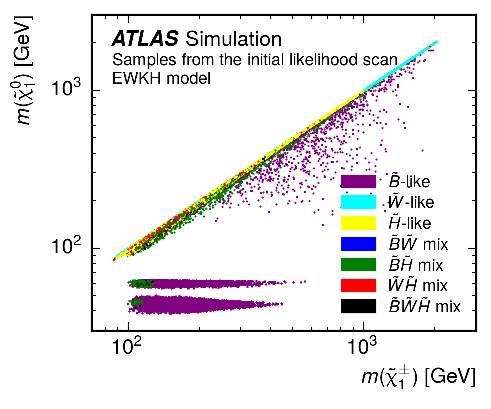
\includegraphics[scale=1.0]{LSP_composition.pdf}
        \caption{The scatter plot in the $m(\widetilde{\chi}^{0}_{1})$ vs $m(\widetilde{\chi}^{\pm}_{1})$ plane~\cite{Aaboud:2016wna}.
        The color encodes the $\widetilde{\chi}^{0}_{1}$ composition.
        The Higgsino-dominated LSPs are colored in yellow and along the $\widetilde{\chi}^{0}_{1}$-$\widetilde{\chi}^{\pm}_{1}$ diagonal.}
        \label{fig:intro_LSP_composition}
    \end{center}
\end{figure}

This dissertation focuses on searching for electroweak production of SUSY particles in compressed scenarios with exactly two low-momentum same-flavor opposite-charged leptons (electron and muon) in final states and missing transverse momentum $\textbf{p}_{\text{T}}^{\text{miss}}$.
This search uses proton-proton collision data at $\sqrt{s} = 13$~{\TeV} recorded by the ATLAS detector at the Large Hadron Collider (LHC)~\cite{Evans:2008zzb} in 2015 and 2016, corresponding to a total integrated luminosity of 36.1~\ifb.
Figure~\ref{fig:intro_feynman_diagrams} shows the Feynman diagrams representing the electroweakino productions with two leptons final state in association with an initial state radiated jet.
Same-flavor opposite-charged leptons come from the $\widetilde{\chi}^{0}_{2}$ decays in the $\widetilde{\chi}^{0}_{2} \widetilde{\chi}^{\pm}_{1}$ and $\widetilde{\chi}^{0}_{2} \widetilde{\chi}^{0}_{1}$ productions, and from the $\widetilde{\chi}^{\pm}_{1}$ decays in the $\widetilde{\chi}^{\pm}_{1} \widetilde{\chi}^{\mp}_{1}$ production.
The two leptons can be reconstructed in the detector and carry small transverse momentum  \pt.
However, the two LSPs are invisible and back-to-back in the rest frame of their parent electroweakinos.
Because they carry large momentum, the missing transverse energy \met is relatively large.
Similar searches have been performed using $\sqrt{s} = 8$~{\TeV} and $\sqrt{s} = 13$~{\TeV} by the ATLAS~\cite{Aad:2014vma, Aad:2014nua, Aad:2015eda, Aaboud:2016wna} and CMS~\cite{Khachatryan:2014qwa, Khachatryan:2015pot, Sirunyan:2017lae} experiments.
Combining with the results from the LEP experiments, the mass limits for sleptons and charginos are $m(\widetilde{e}_{R}) > 73$~{\GeV}, $m(\widetilde{\mu}_{R}) > 94.6$~{\GeV}, and $m(\widetilde{\chi}^{\pm}_{1}) > 103.5$~{\GeV} or 92.4~{\GeV} depending on the $\Delta m(\widetilde{\chi}^{0}_{1}, \widetilde{\chi}^{\pm}_{1})$.

\begin{figure}[htbp]
    \begin{center}
        \begin{subfigure}[b]{0.32\textwidth}
            \begin{center}
                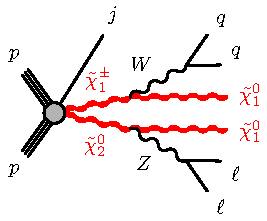
\includegraphics[scale=1.0]{C1N2-llqqN1N1g-WZ.pdf}
                \caption{The $\widetilde{\chi}^{0}_{2} \widetilde{\chi}^{\pm}_{1}$ production.}
            \end{center}
        \end{subfigure}%
        \begin{subfigure}[b]{0.32\textwidth}
            \begin{center}
                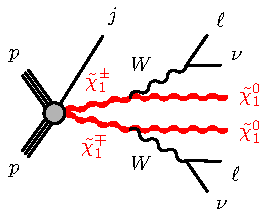
\includegraphics[scale=1.0]{C1C1-llvvN1N1g-WW.pdf}
                \caption{The $\widetilde{\chi}^{\pm}_{1} \widetilde{\chi}^{\mp}_{1}$ production.}
            \end{center}
        \end{subfigure}
        \begin{subfigure}[b]{0.32\textwidth}
            \begin{center}
                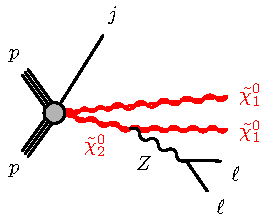
\includegraphics[scale=1.0]{N2N1-jllN1N1-Z.pdf}
                \caption{The $\widetilde{\chi}^{0}_{2} \widetilde{\chi}^{0}_{1}$ production.}
            \end{center}
        \end{subfigure}
    \end{center}
    \caption{The Feynman diagrams representing the two leptons final state of (a) $\widetilde{\chi}^{0}_{2} \widetilde{\chi}^{\pm}_{1}$, (b) $\widetilde{\chi}^{\pm}_{1} \widetilde{\chi}^{\mp}_{1}$, (c) $\widetilde{\chi}^{0}_{2} \widetilde{\chi}^{0}_{1}$ productions.}
    \label{fig:intro_feynman_diagrams}
\end{figure}

This dissertation has the following structure.
An introduction is given in Chapter~\ref{chapter:introduction} followed by theoretical foundations in Chapter~\ref{chapter:standard_model} and \ref{chapter:Supersymmetry}.
The experiment facilities are described in Chapter~\ref{chapter:altas_experiment}.
The data and Monte Carlo samples used are detailed in Chapter~\ref{chapter:data}.
Chapter~\ref{chapter:event_reconstruction_and_selection} presents the event reconstruction and the signal region selection.
The background estimation and the systematic uncertainties are discussed in Chapter~\ref{chapter:bkg_estimation}.
The results and interpretation are reported in Chapter~\ref{chapter:results}.
Finally, the conclusions are summarized in Chapter~\ref{chapter:conclusion}.



\chapter{The Standard Model}
\label{chapter:standard_model}
\graphicspath{{figures/standard_model/}}
This chapter outlines relevant theoretical and mathematical concepts of high energy particle physics.
The Standard Model of particle physics (SM)~\cite{Salam:1968rm, Glashow:1961tr, Weinberg:1967tq, Herrero:1998eq, Cottingham:2007zz} has been developed since the early 1970s and it has successfully explained almost all experimental results.
The SM is well-tested and the most successful physics theory to describe the nature of the elementary particles and their interactions.
An overview of the SM is given in Sect.~\ref{sec:sm}.
Then, some of the open questions are mentioned in Sect.~\ref{sec:sm_bsm}.

%%%
%%%
%%%

\section{The Standard Model of Particle Physics}
\label{sec:sm}
The Standard Model of particle physics is known as the most accurate theory for describing the elementary particles and the interactions between them.
By combining the quantum mechanics and special relativity, the SM is a relativistic \textit{Quantum Field Theory} (QFT) based on a $SU(3)_{C} \otimes SU(2)_{L} \otimes U(1)_{Y}$ symmetry gauge group, where $C$ denotes color, $L$ represents left chirality, and $Y$ stands for weak hypercharge, respectively.
The $SU(3)_{C}$ group is the basis for \textit{Quantum Chromodynamics} (QCD) which describes the strong interaction and the $SU(2)_{L} \otimes U(1)_{Y}$ group is the foundation of the electroweak interaction which unifies the electromagnetic and weak interactions.
Therefore, the SM Lagrangian is invariant under the local gauge transformation.
According to \textit{Noether's Theorem}~\cite{Noether:1918zz}, the invariance of an action of a physical system undergoes a symmetry transformation corresponding to a conservation law and vice versa. 
The gauge invariance of the SM Lagrangian corresponds to the conserved quantum numbers, or the charges, of each interaction.
The conserved charges are the three color charge (red, blue, green) for the strong interaction, the third component of the weak isospin $I_{3}$ for the weak interaction, and the electric charge $Q$ for the electromagnetic interaction.

%%%
%%%
%%%

\subsection{Particle Content}
\label{subsec:sm_particle_content}
According to the SM, all matter around us is made of elementary particles called \textit{quarks} and \textit{leptons}.
The quarks and leptons are called fermions which have half integral spin $s=\frac{1}{2}$, hence the fermions follow the Pauli exclusion principle which says no two fermions have the same quantum state at the same time.
Each fermion has an anti-fermion with the equal mass but carries opposite electric charge, weak isospin and color charge.
There are six quarks and six leptons, they are grouped into three pairs, or "\textit{generations}", ordered by their mass.
The lightest and most stable particles constitute the first generation and they are constituents of ordinary matter.
The heavier and less stable particles form the second and third generations and the heavier particles quickly decay to the next most stable particles.
The three generations of quarks are up ($u$) and down ($d$), charm ($c$) and strange ($s$), and top ($t$) and bottom ($b$) quarks.
The up-type quarks ($u, c, t$) carry $+\frac{2}{3}|e|$ charge and with isospin $+\frac{1}{2}$ while the down-type quarks ($d, s, b$) carry $-\frac{1}{3}|e|$ charge with isospin $-\frac{1}{2}$.
The quarks carry an additional color charge of either red, green, or blue, and hence they only interact via the strong force.
Because the strong force holds quarks together, only non-integer charges of the quark combinations are experimentally allowed.
The quark combinations are called \textit{hadrons} which can be categorized into \textit{mesons} and \textit{baryons}.
The meson is composed by a quark and anti-quark pair ($q\bar{q}$) whereas the baryon is made up by three quarks ($qqq$ or $\bar{q}\bar{q}\bar{q}$).
Only colorless bound states of hadrons are allowed so the quark and anti-quark pair in a meson should contain color and anti-color and the three quarks in a baryon must carry different colors.
The leptons are colorless and are therefore participating in the weak and electromagnetic force only. 
They do not participate in the strong interaction.
The electron-type leptons ($e, \mu, \tau$) carry an elementary charge $|e|$ and their corresponding neutrinos ($\nu_{e}, \nu_{\mu}, \nu_{\tau}$) are neutral.
The neutrinos have very little mass and interact via weak force only.
A summarized table of the properties of quarks and leptons is given in Table~\ref{tab:sm_fermions}.

\begin{table}[htp]
    %\begin{center}
    \resizebox{\textwidth}{!}{% <------ Don't forget this %
        \begin{tabular}{cccccccc}
            \hline
            \hline
            Generation           & Fermion                 &              & particle          & electric charge $Q$ & weak isospin $I_{3}$ & color charge $C$ & mass [{\GeV}]\\
            \hline
            \multirow{4}{*}{I}   & \multirow{2}{*}{Quark}  & $u$          & up quark          & $+\frac{2}{3}|e|$   & $+\frac{1}{2}$       & r,g,b             & 0.0023\\
                                 &                         & $d$          & down quark        & $-\frac{1}{3}|e|$   & $-\frac{1}{2}$       & r,g,b             & 0.0048\\
                                 & \multirow{2}{*}{Lepton} & $e$          & electron          & $-1|e|$             & $-\frac{1}{2}$       & -                 & 0.00051\\
                                 &                         & $\nu_{e}$    & electron neutrino & 0                   & $+\frac{1}{2}$       & -                 & $< 2 \times 10^{-9}$\\
            \hline
            \multirow{4}{*}{II}  & \multirow{2}{*}{Quark}  & $c$          & charm quark       & $+\frac{2}{3}|e|$   & $+\frac{1}{2}$       & r,g,b             & 1.275\\
                                 &                         & $s$          & strange quark     & $-\frac{1}{3}|e|$   & $-\frac{1}{2}$       & r,g,b             & 0.095\\
                                 & \multirow{2}{*}{Lepton} & $\mu$        & muon              & $-1|e|$             & $-\frac{1}{2}$       & -                 & 0.106\\
                                 &                         & $\nu_{\mu}$  & muon neutrino     & 0                   & $+\frac{1}{2}$       & -                 & $< 1.9 \times 10^{-7}$\\
            \hline
            \multirow{4}{*}{III} & \multirow{2}{*}{Quark}  & $t$          & top quark         & $+\frac{2}{3}|e|$   & $+\frac{1}{2}$       & r,g,b             & 173.2\\
                                 &                         & $b$          & bottom quark      & $-\frac{1}{3}|e|$   & $-\frac{1}{2}$       & r,g,b             & 4.18\\
                                 & \multirow{2}{*}{Lepton} & $\tau$       & tau               & $-1|e|$             & $-\frac{1}{2}$       & -                 & 1.777\\
                                 &                         & $\nu_{\tau}$ & tau neutrino      & 0                   & $+\frac{1}{2}$       & -                 & $< 1.82 \times 10^{-5}$\\
            \hline
            \hline
        \end{tabular}
    }
    %\end{center}
    \caption{The Standard Model fermions with charges and masses~\cite{Patrignani:2016xqp}.}
    \label{tab:sm_fermions}
\end{table}%

%\begin{figure}[htbp]
%   \begin{center}
%       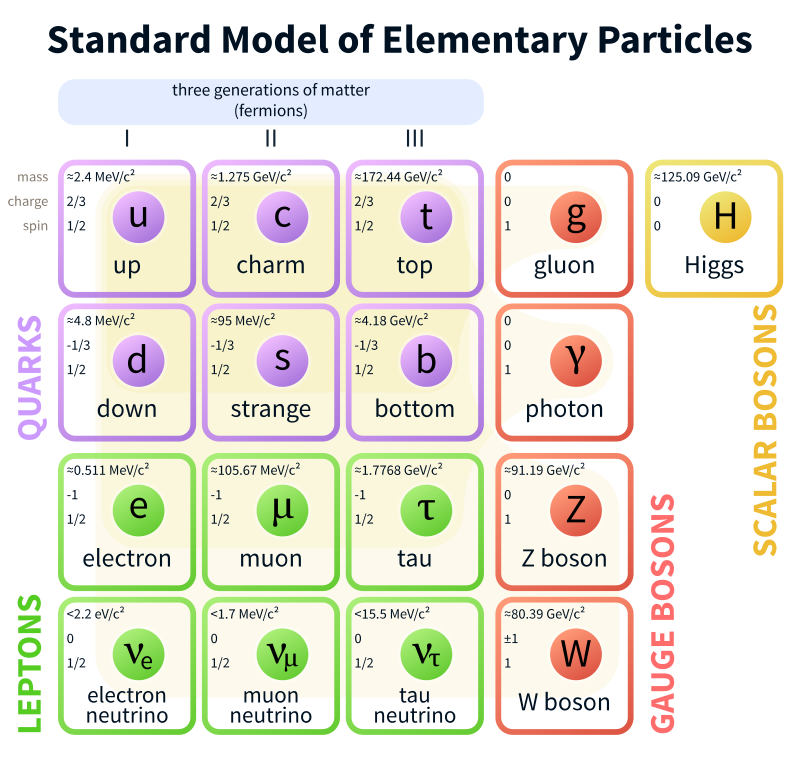
\includegraphics[scale=0.3]{800px-Standard_Model_of_Elementary_Particles.png}
%       \caption{default.
%       https://en.wikipedia.org/wiki/Standard_Model}
%       \label{fig:sm_particles}
%   \end{center}
%\end{figure}

There are four fundamental forces in the universe: the strong force, the weak force, the electromagnetic force, and the gravitational force.
The first three forces are described in the SM, however, the gravitational force could not yet be included in the SM.
Because the effect of the gravitational force is very weak and can be negligible, the SM works well without considering the gravitational force.
Each force has a force-carrier particle called gauge boson and there is a quantum number associate to it.
The gauge bosons of the strong force are eight massless \textit{gluons}, $g$, which associate to color charge $C$.
The gauge bosons of the weak force are $W^{\pm}$ and $Z^{0}$ bosons which associate to weak isospin $I_{3}$.
The gauge boson of the electromagnetic force is massless \textit{photon}, $\gamma$, which associates to electric charge $Q$.
Although the gluon and photon are massless particles, the $W^{\pm}$ and $Z^{0}$ bosons are massive.
The mass of the $W^{\pm}$ and $Z^{0}$ bosons are $m_{W}=80.385 \pm 0.015$~{\GeV} and $m_{Z}=91.1876 \pm 0.0021$~{\GeV}~\cite{Patrignani:2016xqp}, respectively.
Table~\ref{tab:sm_fundamental_forces} shows the four fundamental forces, the relative strength and range together with the theories and the mediators.

\begin{table}[htp]
    %\begin{center}
    \resizebox{\textwidth}{!}{% <------ Don't forget this %
        \begin{tabular}{cccccc}
            \hline
            \hline
            Force           & Rel. Strength & Range [m]  & Theory             & Mediator                     & Mass [{\GeV}]\\
            \hline
            Strong          & $10$          & $10^{-15}$ & Chromodynamics     & Gluon                        & 0\\
            Weak            & $10^{-13}$    & $10^{-18}$ & Flavourdynamics    & $W^{\pm}$ and $Z^{0}$ bosons & 80.4/91.2\\
            Electromagnetic & $10^{-2}$     & $\infty$   & Electrodynamics    & Photon                       & 0\\
            \hline
            Gravitational   & $10^{-42}$    & $\infty$   & General relativity & Graviton                     & -\\
            \hline
            \hline
        \end{tabular}
    }
    %\end{center}
    \caption{The four fundamental forces with the relative strength, interaction range, describing theory, and the mediator with its mass.
    The gravitational force is not a part of the SM and the graviton is a theoretical particle.}
    \label{tab:sm_fundamental_forces}
\end{table}%

%%%
%%%
%%%

\subsection{Local Gauge Theory}
\label{subsec:sm_gauge_theory}
The Lagrangian density of the SM for the free fields\footnote{This is the Lagrangian density of QED. The three terms are fermion kinematic term, photon kinematic term, and interaction, respectively.} listed in the Eq.~(\ref{eq:sm_lagrangian}) is invariant under local gauge transformation\footnote{In Dirac representation, the four contravariant gamma matrices are $\gamma^{0} = \left(\begin{matrix}1 & 0 & 0 & 0\\0 & 1 & 0 & 0\\0 & 0 & -1 & 0\\0 & 0 & 0 & -1\end{matrix}\right)$, $\gamma^{1} = \left(\begin{matrix}0 & 0 & 0 & 1\\0 & 0 & 1 & 0\\0 & -1 & 0 & 0\\-1 & 0 & 0 & 0\end{matrix}\right)$, $\gamma^{2} = \left(\begin{matrix}0 & 0 & 0 & -i\\0 & 0 & i & 0\\0 & i & 0 & 0\\-i & 0 & 0 & 0\end{matrix}\right)$, $\gamma^{3} = \left(\begin{matrix}0 & 0 & 1 & 0\\0 & 0 & 0 & -1\\-1 & 0 & 0 & 0\\0 & 1 & 0 & 0\end{matrix}\right)$}
%
\begin{equation}
    \mathcal{L} = \bar{\psi}(i\gamma^{\mu}\partial_{\mu} - m)\psi + e\bar{\psi}\gamma^{\mu}\psi\bm{A}_{\mu} - \frac{1}{4}\bm{F}_{\mu\nu}\bm{F}^{\mu\nu}
    \label{eq:sm_lagrangian}
\end{equation}
%
where $\bm{F}_{\mu\nu} = \partial_{\mu}\bm{A}_{\nu} - \partial_{\nu}\bm{A}_{\mu}$.
The local gauge transformation means the scalar field $\psi$ and the vector field $\bm{A}_{\mu}$ transform as
%
\begin{align}
    \psi(x) & \rightarrow \psi'(x) = e^{i\theta(x)}\psi(x)\\
    \bm{A}_{\mu}(x) & \rightarrow \bm{A}_{\mu}'(x) = \bm{A}_{\mu}(x) + \frac{1}{e}\partial_{\mu}\theta(x).
    \label{eq:sm_gauge_transformation}
\end{align}
%
By introducing the gauge term, i.e. the vector field, the interacting force can be obtained by calculating the derivatives of the \textit{Euler-Lagrange equations}.
The gauge field can be associated to particular spin one gauge bosons which mediate the force.
The number of the mediating gauge bosons is equal to the dimension of the symmetry group.
From the group theory, the dimension of an unitary group $U(n)$ is $n^{2}$ and the dimension of a special unitary group $SU(n)$ is $n^{2} - 1$.
Because the SM is based on a $SU(3)_{C} \otimes SU(2)_{L} \otimes U(1)_{Y}$ symmetry gauge group, the number of mediators are 8 for $SU(3)_{C}$, 3 for $SU(2)_{L}$, and 1 for $U(1)_{Y}$ corresponding to 8 gluons for the strong interaction, 3 gauge bosons ($W^{\pm}$ and $Z^{0}$) for weak interaction, and 1 photon for the electromagnetic interaction.


%%%
%%%
%%%

\subsection{Strong interaction}
\label{subsec:sm_strong_interaction}
The \textit{Quantum Chromodynamics} (QCD) is the theory to describe the strong interaction.
The gauge bosons are the eight massless gluons which carry three different colors (and anti-colors), red, green, and blue.
Quarks interact with gluons hence they also carry color charge $C$ and can be represented in color triplets
%
\begin{equation}
    \psi = 
    \left(
        \begin{matrix}
            & \psi_{r} & \\
            & \psi_{g} & \\
            & \psi_{b} &
        \end{matrix}
    \right).
    \label{eq:sm_quark_triplets}
\end{equation}
%
The QCD is based on the non-Abelian $SU(3)_{C}$ group which requires local gauge transformation
%
\begin{equation}
    \psi \rightarrow \psi' = e^{i g_{s} \alpha_{a}(x) T^{a}}\psi
    \label{eq:sm_qcd_gauge_transformation_1}
\end{equation}
%
where the $g_{s}$ is the strong coupling constant, $\alpha_{a}(x)$ are arbitrary functions of space-time, and $T^{a}$ are the generators of the non-Abelian $SU(3)_{C}$ group and the summation over $a$ with $a = 1, \dots, 8$ is implied.
The Lagrangian density is invariant under the local gauge transformation by introducing the new form of the gauge fields and the covariant derivative
%
\begin{align}
    \bm{G}_{\mu}^{a} & \rightarrow \bm{G}_{\mu}^{a} -  \partial_{\mu} \alpha^{a}(x) - g_{s} f_{abc} \alpha^{b}(x) \bm{G}_{\mu}^{c} \\
    \partial_{\mu} & \rightarrow D_{\mu} = \partial_{\mu} + i g_{s} T_{a} \bm{G}_{\mu}^{a}
    \label{eq:sm_qcd_gauge_transformation_2}
\end{align}
%
where $f_{abc}$ is the structure constant. 
The Lagrangian density of QCD is given by
%
\begin{equation}
    \mathcal{L}_{QCD} = \bar{\psi}(i \gamma^{\mu} \partial_{\mu} - m) \psi - g_{s} ( \bar{\psi} \gamma^{\mu} T_{a} \psi) \bm{G}_{\mu}^{a} - \frac{1}{4} \bm{G}_{\mu\nu}^{a} \bm{G}_{a}^{\mu\nu}
    \label{eq:sm_qcd_lagrangian}
\end{equation}
%
where the field strength tensor $\bm{G}_{\mu\nu}^{a} = \partial_{\mu} \bm{G}_{\nu}^{a} - \partial_{\nu} \bm{G}_{\mu}^{a} - g_{s} f_{abc} \bm{G}_{\mu}^{b} \bm{G}_{\nu}^{c}$ causing self-interactions between the gluons.
The strong force increases with distance between quarks, therefore, the quarks exist only as colorless compounds such as meson or baryon mentioned in Sect.~\ref{subsec:sm_particle_content}.
The production of a single quark is accompanied by the creation of an anti-quark from vacuum to form a quark and anti-quark pair as a colorless compound.
This is called \textit{hadronisation}.
The phenomena that confined quarks in the small interaction range is called \textit{confinement}.
But at small distance or high energy, the quarks can be considered as quasi-free particles.
This is referred to as \textit{asymptotic freedom}.

%%%
%%%
%%%

\subsection{Electroweak interaction}
\label{subsec:sm_ewk_interaction}
Fermi formulated the first weak interaction theory in 1933~\cite{Fermi:1934hr}, however, the theory only holds for energies less than 100~{\GeV}.
Glashow, Salam, and Weinberg (GSW) proposed a new model~\cite{Salam:1968rm, Weinberg:1967tq, Glashow:1961tr} which unifies electromagnetic and weak forces to become \textit{electroweak} (EW) force and this new \textit{GSW model} can apply to the energy greater than 100~{\GeV}.
The electroweak theory is based on $SU(2)_{L} \otimes U(1)_{Y}$ gauge symmetry where the subscripts $L$ denotes the left-handedness because only the left-handed fermions (and right-handed anti-fermions) and $Y$ denotes the weak hypercharge, a new quantum number, which relates to the electric charge $Q$ and the weak isospin $I_{3}$ by the \textit{Gell-Mann-Nishijima relation}~\cite{Nakano:1953zz, Gell-Mann:1956iqa}
%
\begin{equation}
    Y = 2(Q - I_{3}).
    \label{eq:sm_hypercharge}
\end{equation}
%
The left-handed and right-handed fermion field $\psi$ can be decomposed into two components
%
\begin{align}
    \psi & = P_{L}\psi + P_{R}\psi\\
         & = \psi_{L} + \psi_{R}
    \label{eq:sm_fermion_field_components}
\end{align}
%
where the projection operators $P_{L}$ and $P_{R}$ are defined as\footnote{$\gamma^{5}$ is the product of the four gamma matrices. $\gamma^{5} = i \gamma^{0} \gamma^{1} \gamma^{2} \gamma^{3} = \left(\begin{matrix}0 & 0 & 1 & 0\\0 & 0 & 0 & 1\\1 & 0 & 0 & 0\\0 & 1 & 0 & 0\end{matrix}\right)$}
%
\begin{align}
    P_{L} & = \frac{1}{2} (1 - \gamma^{5})\\
    P_{R} & = \frac{1}{2} (1 + \gamma^{5}).
    \label{eq:sm_projection_operators}
\end{align}
%
The projection operators satisfy $P_{L}P_{R} = 0$ and $P_{L} + P_{R} = 1$.
Experimental observations show the right-handed neutrinos don't participate in all the interactions described in the SM so the $\psi_{R}$ is a singlet and $I_{3} = 0$\footnote{The left-handed fermion state $\psi_{L}$ is a doublet.}.
The local gauge transformations of the $SU(2)_{L} \otimes U(1)_{Y}$ are
%
\begin{align}
    \psi_{L} & \rightarrow \psi_{L}' = e^{i \alpha_{a}(x) T^{a}}e^{i \beta(x) Y} \psi_{L}\\
    \psi_{R} & \rightarrow \psi_{R}' = e^{i \beta(x) Y} \psi_{R}
    \label{eq:sm_local_gauge_transformations_ew_1}
\end{align}
%
where $T^{a} = \frac{\sigma^{a}}{2}$ are the generators of $SU(2)_{L}$ with Pauli matrix $\sigma^{a}$\footnote{The Pauli matrices are $\sigma_{1}=\left(\begin{matrix}0 & 1\\1 & 0\end{matrix}\right)$, $\sigma_{2}=\left(\begin{matrix}0 & -i\\i & 0\end{matrix}\right)$, and $\sigma_{3}=\left(\begin{matrix}1 & 0\\0 & -1\end{matrix}\right)$} and $Y$ is the generator of $U(1)_{Y}$.
The $\alpha_{a}(x)$ and $\beta(x)$ depend on the space-time.
The covariant derivative with respect to the $SU(2)_{L} \otimes U(1)_{Y}$ is
%
\begin{equation}
    D_{\mu} = \partial_{\mu} + i g_{W} T_{a} \bm{W}_{\mu}^{a} + i g_{Y} Y \bm{B}_{\mu}
    \label{eq:sm_derivative_ew}
\end{equation}
%
where $g_{W}$ and $g_{Y}$ are coupling constants and $\bm{W}_{\mu}^{a}$ ($a = 1, 2, 3$) and $\bm{B}_{\mu}$ are the gauge fields.
The gauge fields $\bm{W}_{\mu}^{a}$ and $\bm{B}_{\mu}$ transform under the $SU(2)_{L} \otimes U(1)_{Y}$ symmetry as
%
\begin{align}
    \bm{W}_{\mu}^{a} & \rightarrow \bm{W}_{\mu}^{a} - \frac{1}{g_{W}} \partial_{\mu} \alpha^{a}(x) - \epsilon^{abc} \alpha^{b}(x) \bm{W}_{\mu}^{c}\\
    \bm{B}_{\mu} & \rightarrow \bm{B}_{\mu} - \frac{1}{g_{Y}} \partial_{\mu} \beta(x)
    \label{eq:sm_local_gauge_transformations_ew_2}
\end{align}
%
where $\epsilon^{abc}$ is the Levi-Civita tensor.
The Lagrangian density of the electroweak is given by
%
\begin{equation}
    \mathcal{L}_{EW} = \bar{\psi}_{L} (i \gamma^{\mu} D_{\mu} - m) \psi_{L} + \bar{\psi}_{R} (i \gamma^{\mu} D_{\mu} - m) \psi_{R} - \frac{1}{4} \bm{W}_{\mu\nu}^{a} \bm{W}_{a}^{\mu\nu} - \frac{1}{4} \bm{B}_{\mu\nu} \bm{B}^{\mu\nu}
    \label{eq:sm_Lagrangian_ew}
\end{equation}
%
where $\bm{W}_{\mu\nu}^{a}$ and $\bm{B}_{\mu\nu}$ are the field strength tensors
%
\begin{align}
    \bm{W}_{\mu\nu}^{a} & = \partial_{\mu} \bm{W}_{\nu}^{a} - \partial_{\nu} \bm{W}_{\mu}^{a} - g_{W} \epsilon^{abc} \bm{W}_{\mu}^{b} \bm{W}_{\nu}^{c}\\
    \bm{B}_{\mu\nu} & = \partial_{\mu} \bm{B}_{\nu} - \partial_{\nu} \bm{B}_{\mu}
    \label{eq:sm_field_strangth_tensors}
\end{align}
%
and $\bar{\psi} \equiv \psi^{\dagger} \gamma^{0}$ is the adjoint spinor of $\psi$\footnote{$\psi^{\dagger}$ is the hermitian conjugate of $\psi$}.
Therefore, the mass eigenstates are the mixture of the gauge fields
%
\begin{align}
    \bm{W}_{\mu}^{\pm} & = \frac{1}{\sqrt{2}} (\bm{W}_{\mu}^{1} \mp i \bm{W}_{\mu}^{2})\\
    \left(\begin{matrix}\bm{A}_{\mu}\\\bm{Z}_{\mu}\end{matrix}\right) & = \left(\begin{matrix}\cos\theta_{W} & \sin\theta_{W}\\-\sin\theta_{W} & \cos\theta_{W} \end{matrix}\right) \left(\begin{matrix}\bm{B}_{\mu}\\\bm{W}_{\mu}^{3}\end{matrix}\right).
    \label{eq:sm_mass_eigenstates}
\end{align}
%
Thus, the mass eigenstates $\bm{A}_{\mu}$, $\bm{W}_{\mu}^{\pm}$, and $\bm{Z}_{\mu}$ are identified as the photon, $\gamma$, $W^{\pm}$ and $Z^{0}$ bosons experimentally.
The \textit{Weinberg weak mixing angle} $\theta_{W}$ is defined as
%
\begin{equation}
    \tan \theta_{W} = \frac{g_{Y}}{g_{W}}.
    \label{eq:sm_mixing_angle}
\end{equation}
%
The coupling constants $g_{W}$ and $g_{Y}$ are related to the electric charge by
%
\begin{equation}
    e = g_{W} \sin\theta_{W} = g_{Y} \cos\theta_{Y}.
    \label{eq:sm_coupling_constants}
\end{equation}
%
And the weak eigenstates of quark, $q'$, are the linear combinations of the mass eigenstates of quark, q, by the \textit{Cabbibo-Kobayashi-Maskawa} (CKM) matrix~\cite{Kobayashi:1973fv}
%
\begin{equation}
    \left(\begin{matrix}d'\\s'\\b'\end{matrix}\right) = \left(\begin{matrix}V_{ud} & V_{us} & V_{ub}\\V_{cd} & V_{cs} & V_{cb}\\V_{td} & V_{ts} &V_{tb}\end{matrix}\right) \left(\begin{matrix}d\\s\\b\end{matrix}\right).
    \label{eq:sm_CKM_matrix}
\end{equation}
%
The CKM matrix allows the quarks changing their flavor and generation as observed in the experiment.
Similarly, the \textit{Pontecorvo-Maki-Nakagawa-Sakata} (PMNS) matrix~\cite{Maki:1962mu} is responsible for the flavor changing of the neutrinos.

%%%
%%%
%%%

\subsubsection{Spontaneous symmetry breaking and Higgs mechanism}
\label{subsubsec:sm_Higgs_mechanism}
The gauge bosons of the weak interaction, $W^{\pm}$ and $Z^{0}$, are massive particles\footnote{$m_{W}=80.385 \pm 0.015$~{\GeV} and $m_{Z}=91.1876 \pm 0.0021$~{\GeV}}.
However, the existence of the mass terms violate the gauge invariance of the $\mathcal{L}_{EW}$.
In order to explain the mass of gauge bosons, the Englert-Brout-Higgs mechanism~\cite{Higgs:1966ev, Higgs:1964pj, Higgs:1964ia, Englert:1964et, Guralnik:1964eu} was proposed in 1964.
A new scalar complex $SU(2)_{L}$ doublet field $\Phi$ is introduced in the Higgs mechanism
%
\begin{equation}
    \Phi = \left(\begin{matrix}\Phi^{+}\\\Phi^{0}\end{matrix}\right) = \left(\begin{matrix}\Phi_{1} & i\Phi_{2}\\\Phi_{3} & i\Phi_{4}\end{matrix}\right)
    \label{eq:sm_higgs_doublet}
\end{equation}
%
with hypercharge $Y = 1$ and four degrees of freedom, $\Phi_{i}$, which are scalar fields and called the \textit{Goldstone modes}.
The Lagrangian density for this new field, Higgs field, is
%
\begin{equation}
    \mathcal{L}_{\Phi} = (D^{\mu}\Phi)^{\dagger}(D_{\mu}\Phi) - V(\Phi)
    \label{eq:sm_higgs_lagrangian}
\end{equation}
%
where the Higgs potential is defined as
%
\begin{equation}
    V(\Phi) = \mu^{2}|\Phi|^{2} + \lambda|\Phi|^{4}
    \label{eq:sm_higgs_potential}
\end{equation}
%
where $\mu$ and $\lambda$ are free parameters.
The Higgs potential is shown in Fig.~\ref{fig:sm_higgs_potential}.
The Higgs potential is the rotation $U(1)$ symmetry.
Choosing any of the points at the bottom of the Higgs potential breaks the symmetry spontaneously.
The \textit{spontaneously symmetry breaking} (SSB) means the Lagrangian keeps invariant under certain symmetry but no longer invariant at the ground state.

\begin{figure}[htbp]
    \begin{center}
        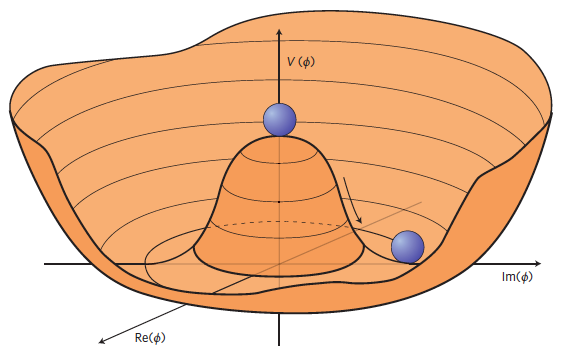
\includegraphics[scale=0.4]{higgspotential.png}
        \caption{An illustration of the Higgs potential which has the form of a ``Mexican hat''~\cite{Ellis:2013jnq}.}
        \label{fig:sm_higgs_potential}
    \end{center}
\end{figure}

Because the Higgs potential is invariant under $SU(2)_{L} \otimes U(1)_{Y}$, the parameters $\mu$ and $\lambda$ must satisfy $\mu^{2} < 0$ and $\lambda > 0$ resulting in a set of degenerate ground states where $\langle 0|\Phi|0 \rangle \neq 0$.
Among the degenerate ground states, the ground state is often chosen to have the form
%
\begin{equation}
    \Phi = \frac{1}{\sqrt{2}}\left(\begin{matrix}0\\v\end{matrix}\right)
    \label{eq:sm_ground_state}
\end{equation}
%
where $v = \sqrt{-\mu^{2}/\lambda}$ is the \textit{the vacuum expectation value} (VEV).
This particular choice of the ground state breaks the $SU(2)_{L} \otimes U(1)_{Y}$ symmetries spontaneously and  ensures the unbroken electromagnetic interaction under $U(1)_{EM}$ symmetry and photon being massless.
By introducing a massive particle, Higgs boson $H$, the Higgs field can be re-written as
%
\begin{equation}
    \Phi = \frac{1}{\sqrt{2}}\left(\begin{matrix}0\\v + H\end{matrix}\right)
    \label{eq:sm_ground_state_2}
\end{equation}
%
and the kinematic term of the Lagrangian density becomes
%
\begin{align}
    \mathcal{L}_{\Phi}^{\textrm{kinematic}} & = (D^{\mu}\Phi)^{\dagger}(D_{\mu}\Phi)\\
                                            & = \frac{1}{2}\partial_{\mu}H\partial^{\mu}H + (v + H)^{2}\Big\{\frac{g_{W}^{2}}{4} \bm{W}_{\mu}^{\dagger}\bm{W}^{\mu} + \frac{g_{W}^{2}}{8\cos^{2}\theta_{W}}\bm{Z}_{\mu}^{\dagger}\bm{Z}^{\mu}\Big\}
    \label{eq:sm_Lagrangian_kinematic_term}
\end{align}
%
and the Higgs potential is now
%
\begin{equation}
    V(\Phi) = -\frac{v^{2} \lambda}{2}(v+H)^{2} + \frac{\lambda}{4}(v+H)^{4}.
\end{equation}
%
Thus the masses of the $W^{\pm}$ and $Z^{0}$ are obtained by the interaction between the gauge bosons and Higgs boson.
The masses are defined as
%
\begin{equation}
    m_{H} = v\sqrt{2\lambda}, \quad m_{W} = \frac{v}{2}g_{W}, \quad m_{Z} = \frac{v}{2}\sqrt{g_{W}^{2} + g_{Y}^{2}}, \quad m_{\gamma} = 0.
\end{equation}
%
However, the masses of fermions are obtained by the \textit{Yukawa interaction}
%
\begin{equation}
    \mathcal{L}_{\textrm{Yukawa}} = y_{f} \bar{L}_{L} \Phi f_{R} + y_{f} \bar{Q}_{L} \Phi f_{R} + \textrm{h.c.}
\end{equation}
%
where the $y_{f}$ is \textit{Yukawa coupling}, $f$ stands for \{$\ell^{i}$, $u^{i}$, $d'^{i}$\} and h.c. represents the hermitian conjugate, respectively.
The $\bar{L}_{L}$ and $\bar{Q}_{L}$ are the left-handed lepton and quark doublet and $f_{R}$ is the lepton or quark singlet.
The mass of fermion is defined as
%
\begin{equation}
    m_{f} = \frac{v}{\sqrt{2}}y_{f}
\end{equation}
%
where $y_{f}$ is a free parameter which causes the fermion mass not predictable.
Finally, the non-zero VEV, $v$, can be related to \textit{Fermi constant}, $G_{F}$, by
%
\begin{equation}
    v = \frac{1}{\sqrt{\sqrt{2} G_{F}}} \approx 246 \textrm{~{GeV}}.
\end{equation}
%

%%%
%%%
%%%

\subsection{The discovery of Higgs boson}
A lot of the SM predictions are successfully confirmed by the experimental observations besides the existence of the theoretical Higgs boson. 
The search of the Higgs boson has become a major goal of the experimental particle physicists.
A Higgs-like resonance was discovered and announced on July 4th 2012 by the ATLAS\footnote{A Toroidal LHC ApparatuS} and CMS\footnote{Compact Muon Solenoid} collaborations~\cite{Aad:2012tfa, Chatrchyan:2012xdj}.
By combining the data with integrated luminosities of 4.8~{\ifb} collected at $\sqrt{s} = 7$~{\TeV} in 2011 and 5.8~{\ifb} at $\sqrt{s}=8$~{\TeV} in 2012, the ATLAS experiment measured the mass of the Higgs boson to be $126.0 \pm 0.4$ (stat.) $\pm 0.4$ (syst.)~{\GeV} with significance of 5.9$\sigma$ corresponding to a background fluctuation probability of $1.7 \times 10^{-9}$~\cite{Aad:2012tfa}.
In the meantime, the CMS experiment announced the mass of the Higgs boson to be $125.3 \pm 0.4$ (stat) $\pm 0.5$ (syst.)~{\GeV} with significance 5.0$\sigma$ using integrated luminosities of up to 5.1~{\ifb} at 7 TeV and 5.3~{\ifb} at 8 TeV~\cite{Chatrchyan:2012xdj}. 
The $H \rightarrow ZZ^{(*)} \rightarrow 4\ell$, $H \rightarrow \gamma \gamma$, and $H \rightarrow WW^{(*)} \rightarrow e\nu\mu\nu$ channels were studied by the ATLAS collaboration and the $H \rightarrow \gamma \gamma, ZZ, W^{+}W^{-}, \tau^{+}\tau^{-}$, and $b\bar{b}$ channels were studied by the CMS collaboration.
In the Fig.~\ref{fig:sm_discovery_of_Higgs} shows the local $p$-value as a function of the Higgs mass for ATLAS and CMS results, respectively.

\begin{figure}[htbp]
    \begin{center}
        \begin{subfigure}[b]{0.48\textwidth}
            \begin{center}
                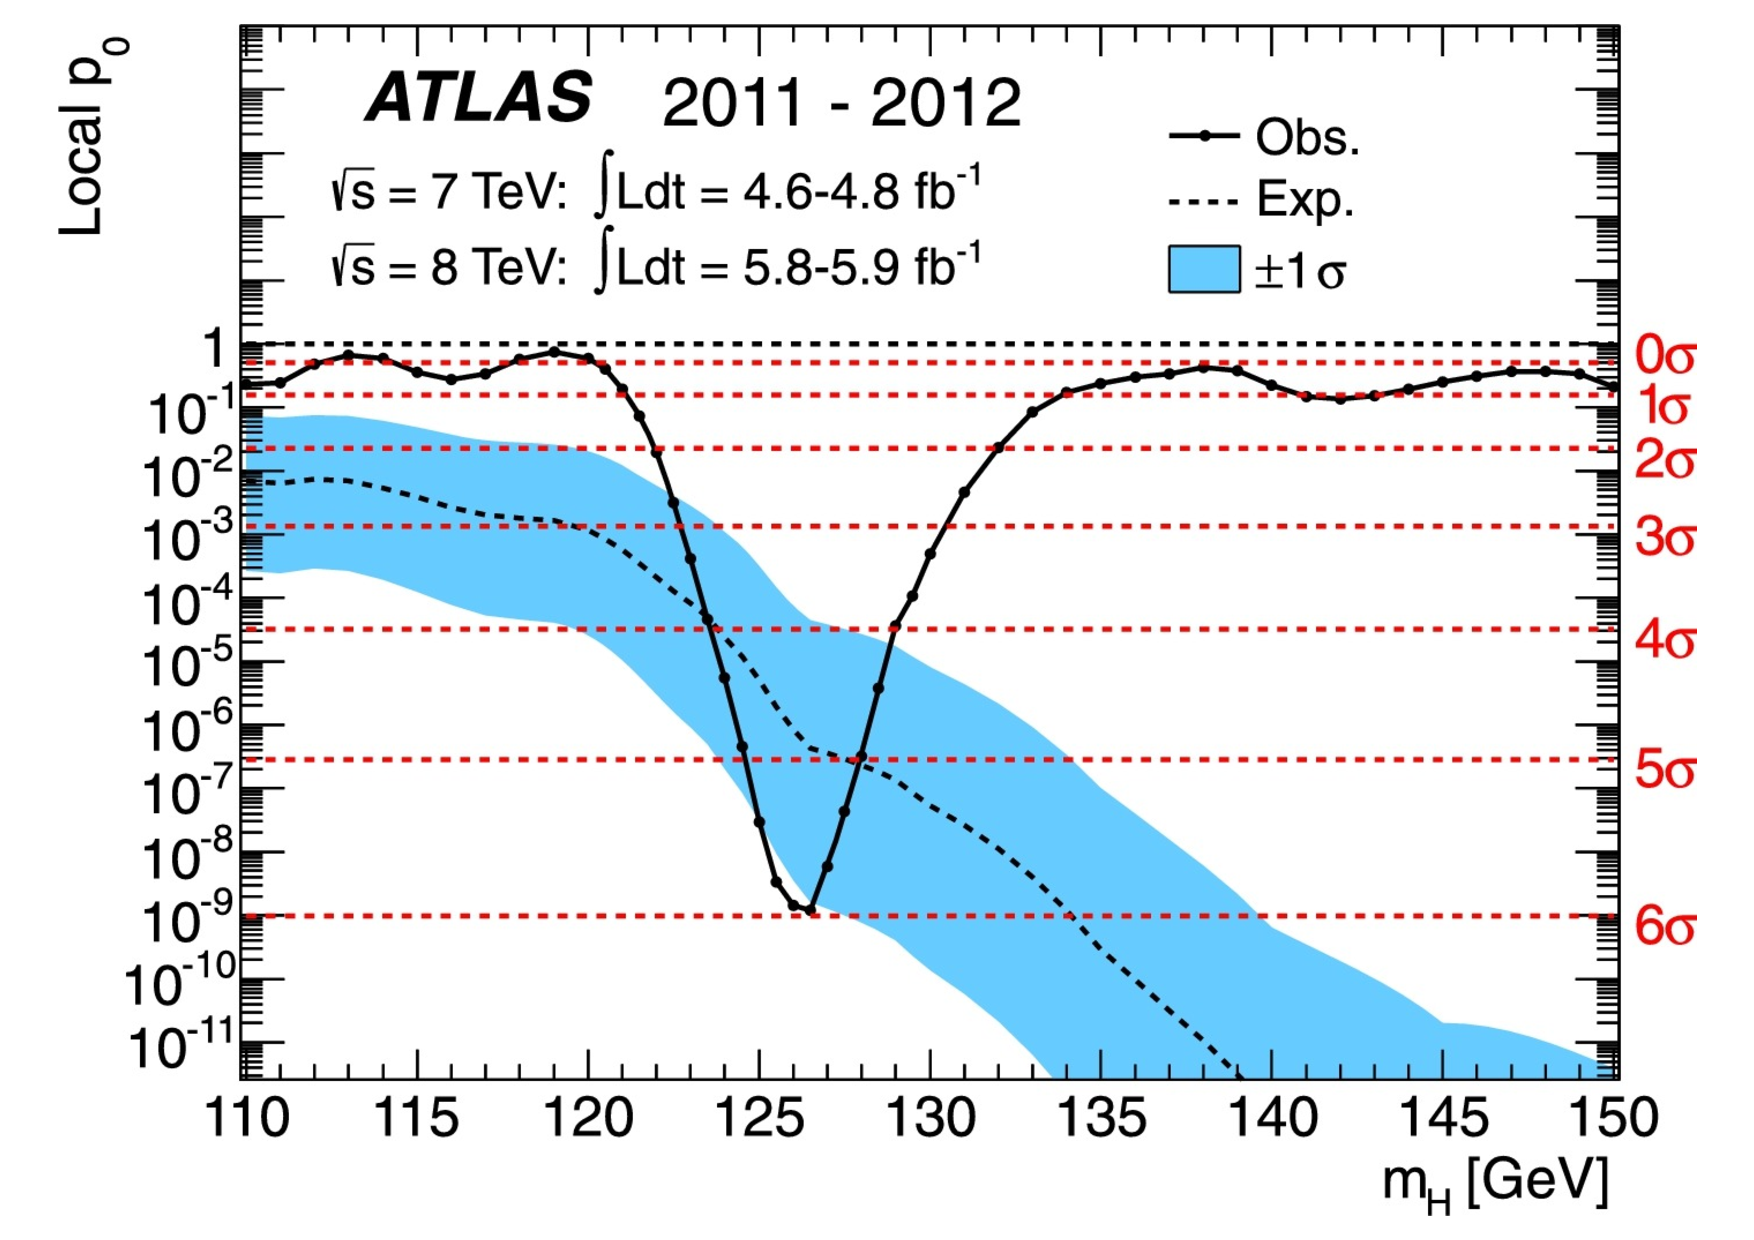
\includegraphics[scale=0.23]{1-s2_0-S037026931200857X-gr009_lrg.pdf}
                \caption{ATLAS results}
            \end{center}
        \end{subfigure}%
        \begin{subfigure}[b]{0.48\textwidth}
            \begin{center}
                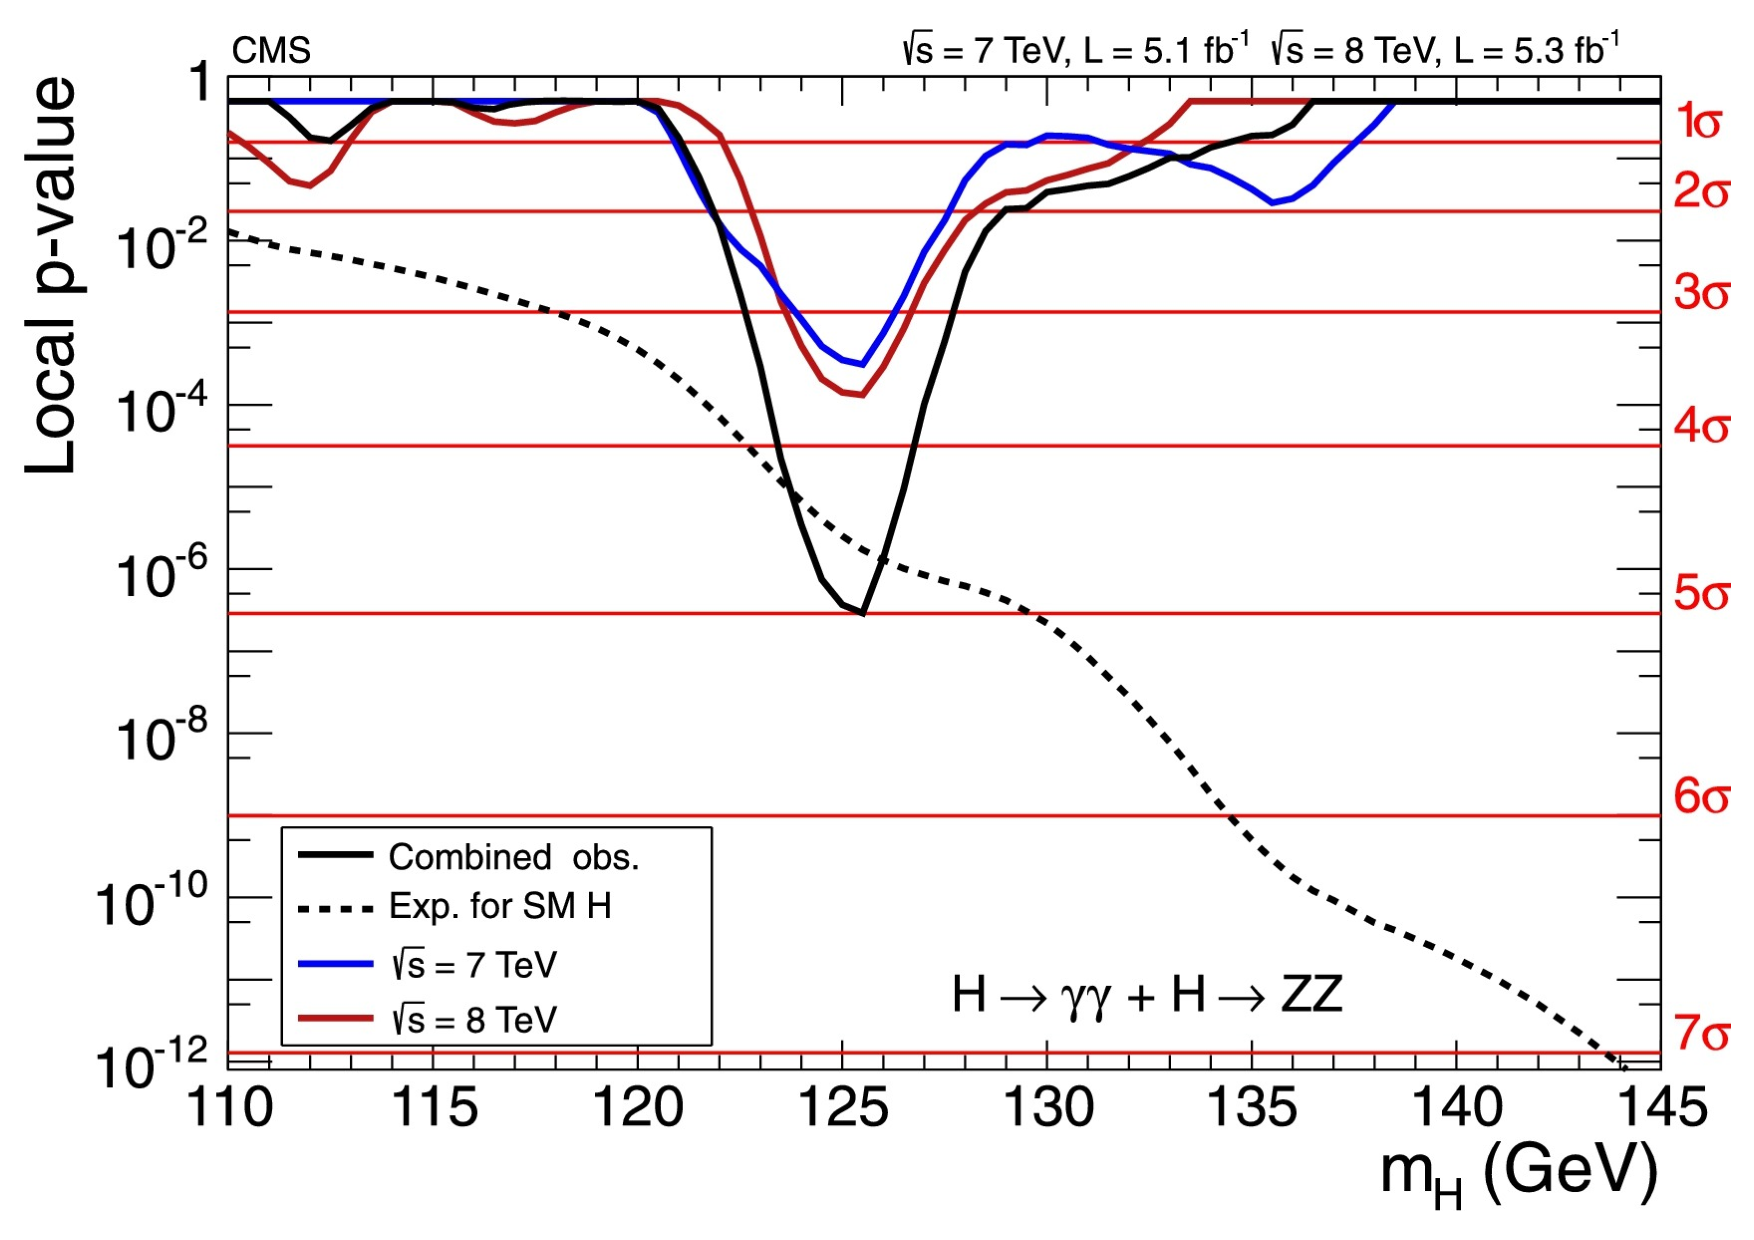
\includegraphics[scale=0.23]{1-s2_0-S0370269312008581-gr016_lrg.pdf}
                \caption{CMS results}
            \end{center}
        \end{subfigure}
    \end{center}
    \caption{The observed local $p$-value as a function of \mH for the ATLAS~\cite{Aad:2012tfa} and CMS~\cite{Chatrchyan:2012xdj} experiment, respectively.
    The dashed line shows the expected local $p_{0}$ for a SM Higgs boson.
    The horizontal lines denotes the $p$-values corresponding to significances of 1 to 6$\sigma$.}
    \label{fig:sm_discovery_of_Higgs}
\end{figure}

%%%
%%%
%%%

\section{Beyond the Standard Model}
\label{sec:sm_bsm}
Although the SM is an incredible successful theory for explaining the phenomenon in the particle physics, it leaves some questions which can no be answered.
Some of the unanswered questions are introduced in the rest part of this section.

%%%
%%%
%%%

\subsection{Hierarchy problem}
\label{subsec:sm_hierarchy_problem}
The weakest force in the SM is the weak force but the strength of the weak force is $10^{24}$ times as strong as gravitational force which doesn't incorporate into the SM.
The large discrepancy between the weak force and the gravitational force is called the hierarchy problem~\cite{Martin:1997ns, Chankowski:1998za, maarten_brak}.
The classical potential of the SM Higgs field $\Phi$ is
%
\begin{equation}
    V(\Phi) = \mu^{2} |\Phi|^2 + \lambda |\Phi|^4.
\end{equation}
%
Since the SM requires the VEV for $\Phi$, $\langle \Phi \rangle$, at the minimum of the potential non-vanishing, this only satisfied if $\mu^{2} < 0$ and $\lambda > 0$.
However, the parameter $\mu^{2}$ receives enormous radiative corrections causing it ultraviolet divergent as shown in Eq.~(\ref{eq:sm_mu2_correction}).
%
\begin{equation}
    \mu^{2} = \mu_{bare}^{2} - \frac{|\lambda_{f}|^{2}}{8\pi}\Lambda_{UV}^{2} + \mathcal{O}(\Lambda_{UV}^{2})
    \label{eq:sm_mu2_correction}
\end{equation}
%
where $\mu_{bare}$ is the Higgs mass, $- \frac{|\lambda_{f}|^{2}}{8\pi}\Lambda_{UV}^{2}$ is the one-loop correction, and $\Lambda_{UV}$ is an ultraviolet momentum cutoff which is valid up to the Plank scale $10^{19}$~{\GeV}.
The electroweak gauge bosons $W^{\pm}$ and $Z^{0}$ obtain their finite masses from $\langle \Phi \rangle$ so the $\mu^{2}$ cannot be divergent.
There must some unknown mechanism to protect from divergence.

%%%
%%%
%%%

\subsection{Dark matter and dark energy}
\label{subsec:sm_dm}
The matters we know today compose of only 5\%~\cite{Bennett:2012zja, Ade:2013sjv} of the content of the universe and the remaining part is something we don't know.
This unknown matter is called \textit{Dark Matter} (DM)~\cite{Bertone:2004pz} which makes up about 27\% of the universe and the rest 68\% are called \textit{Dark Energy} (DE)~\cite{Bennett:2012zja, Ade:2013sjv}.
Because DM interacts weakly and doesn't interact with the electromagnetic force, it doesn't absorb, emit, or reflect light causing it hard to detect directly. 
The name DM comes from it is invisible.
Dark energy distributes evenly in both space and time throughout the universe so it doesn't dilute when the universe expands.
The observed scientific data hints the presence of DE is necessary to explain the accelerated expansion of the universe.

%%%
%%%
%%%

\subsection{Grand Unification}
\label{subsec:sm_grand_unification}

\begin{figure}[tbp]
    \begin{center}
        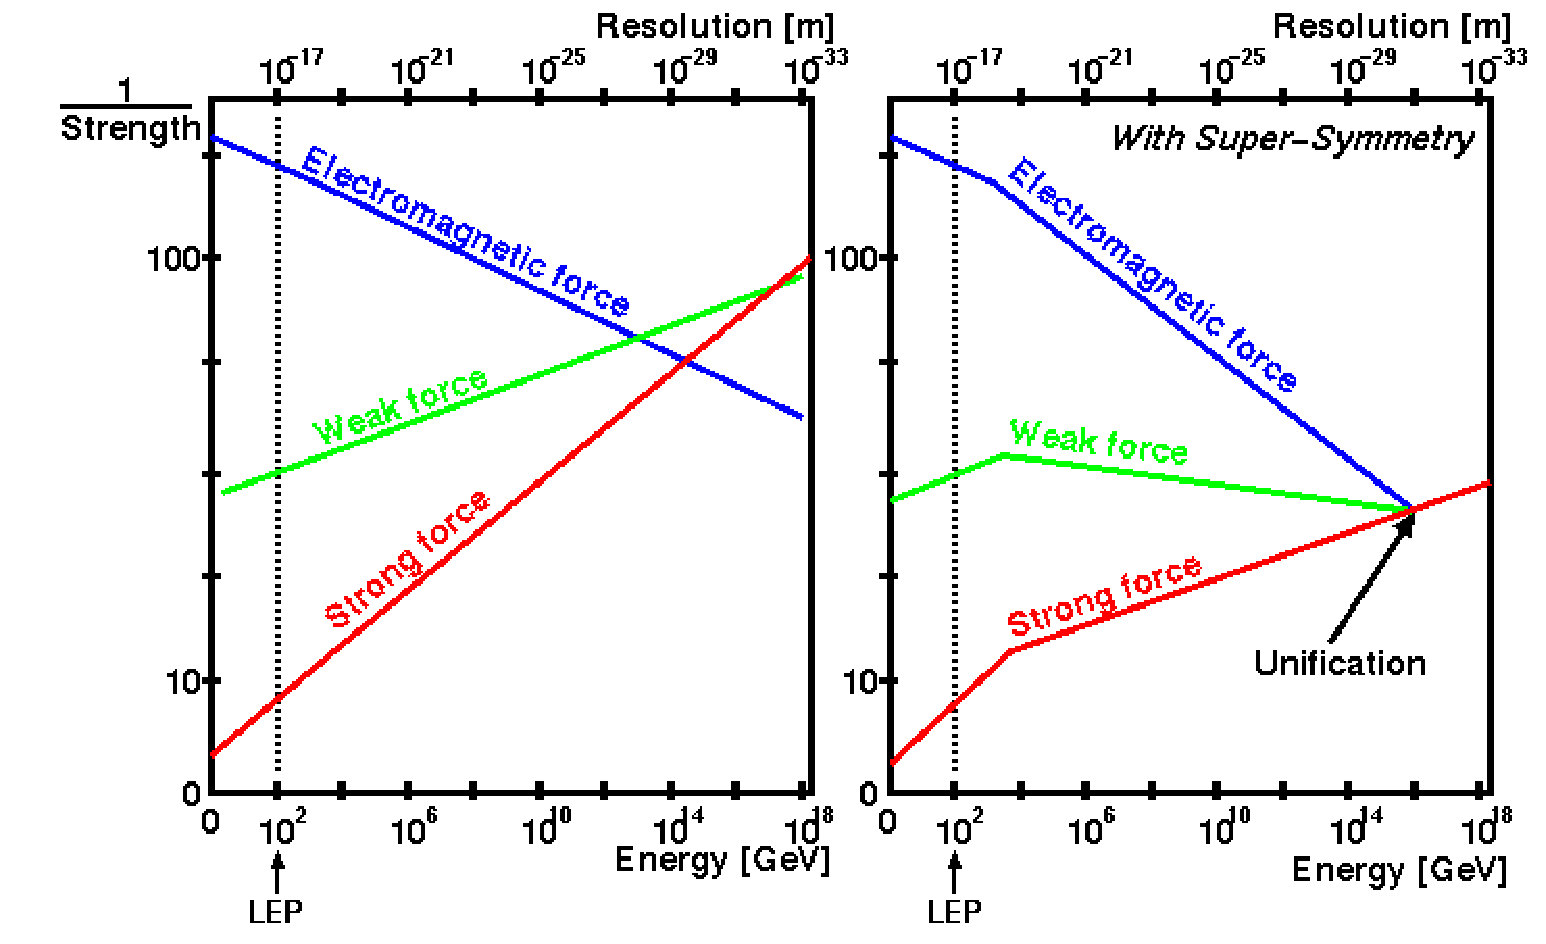
\includegraphics[scale=0.46]{running_coupling.pdf}
        \caption{The measured running coupling constants in the SM (left) and prediction in the GUT (right)~\cite{Ur0ol}.
        The three lines show the inverse value of the coupling constant for the three fundamental forces.}
        \label{fig:sm_coulping_constants}
    \end{center}
\end{figure}

Maxwell unified the electricity and magnetism into electromagnetism in the 1860s.
About a century later, physicists successfully developed theory of electroweak which links the electromagnetism and the weak force.
Because of the triumph of electroweak theory, theorists raise the question of the possibility to unify all forces.
The \textit{Grand Unified Theory} (GUT)~\cite{Ross:1985ai}, which tries to link three of the four known forces together, is developed in the mid-1970s by theorists
The GUT proposes that the electromagnetic force, weak force, and strong force unify to one force at the GUT scale, $\Lambda_{GUT} \approx 10^{16}$~{\GeV}.
So the three running coupling constants~\cite{Mohr:2015ccw} are expected to be converged at the GUT scale.
However, the current experiment results show the coupling constants still different as shown in Fig.~\ref{fig:sm_coulping_constants}.

%%%
%%%
%%%

\subsection{More questions}
\label{subsec:sm_more_questions}
There are some more interesting questions which we don't know the answers.
For example, we don't know the reason why there are 61 elementary particles and more than 20 arbitrary parameters in the SM.
Also, the SM doesn't explain why there are only three generations.
The amount of matter and anti-matter are equal at the beginning of the universe based on the prediction of the SM but the matter dominates in the currently universe which the SM couldn't answer the reason why.

In order to answer these questions, there are many theories being developed on the top of SM but none of them has been observed.
One of the most probable candidate for answering these question is supersymmetry which will be introduced in the next chapter.



\chapter{Suppersymmetry}
\label{chapter:Suppersymmetry}
\graphicspath{{figures/Suppersymmetry/}}
\input{chapter_Suppersymmetry}


\chapter{The ATLAS Experiment at LHC}
\label{chapter:altas_experiment}
\graphicspath{{figures/atlas_experiment/}}
The European Organization for Nuclear Research (CERN\footnote{The name CERN is derived from the acronym for the French Conseil Europ\'{e}en pour la Recherch Nucl\'{e}aire}) was founded in 1954 and is based in the suburb of Geneva on the Franco\textendash Swiss border.
The main function of CERN is to provide particle accelerators and detectors for high-energy physics research.
The physicists and engineers at CERN are probing the fundamental structure of the universe using the world's largest and most complex scientific facility \textemdash \ the Large Hadron Collider (LHC)~\cite{1748-0221-3-08-S08001}.
In the LHC, the particles are boosted to high energies and collide at close to the speed of light.
The results of the collisions are recorded by the various detectors.
There are seven experiments at the LHC.
The biggest of these experiments are ATLAS (A Toroidal LHC ApparatuS)~\cite{1748-0221-3-08-S08003} and CMS (Compact Muon Solenoid)~\cite{1748-0221-3-08-S08004} which use general-purpose detectors to investigate a broad physics programme ranging from the search for the Higgs boson to extra dimensions and particles that could make up dark matter.
The ALICE (A Large Ion Collider Experiment)~\cite{1748-0221-3-08-S08002} experiment is designed to study the physics of quark-gluon plasma form and the LHCb (Large Hadron Collider beauty)~\cite{1748-0221-3-08-S08005} experiment specializes in investigating of CP violation by studying the $b$-quark.
These four detectors sit underground in huge caverns of the LHC ring.
The rest three experiments, TOTEM~\cite{1748-0221-3-08-S08007}, LHCf~\cite{1748-0221-3-08-S08006}, and MoEDAL~\cite{Pinfold:1181486}, are smaller.
The TOTEM (TOTal Elastic and diffractive cross section Measurement)~\cite{1748-0221-3-08-S08007} experiment aims at the measurement of total cross section, elastic scattering, and diffractive dissociation.
The LHCf (Large Hadron Collider forward)~\cite{1748-0221-3-08-S08006} experiment is intended to measure the neutral particle produced by the collider using the forward particles.
The prime motivation of the MoEDAL (Monopole and Exotics Detector at the LHC)~\cite{Pinfold:1181486} experiment is to search directly for the magnetic monopole.

\section{The Large Hadron Collide}

The LHC~\cite{1748-0221-3-08-S08001} is the world's largest and most powerful accelerator which accelerates and collides protons in a 26.7~km circumference crossing the Franco\textendash Swiss border 100 m underground.
Built in the tunnel of the former LEP (Large Electron\textendash Positron), the LHC is capable of colliding protons as well as heavy ions.
Comparing with the LEP which collides electrons and positrons, the advantage of the LHC is the lower energy loss \footnote{The energy loss for protons is about eleven orders of magnitude smaller than the electrons} in the synchrotron radiation, such that higher energies can be reached by the LHC.
The LHC is designed for collisions at a centre-of-mass energy $\sqrt{s}=14$~{\TeV} and an instantaneous luminosity of $\mathcal{L} =10^{34}~\textrm{cm}^{-2}\textrm{s}^{-1}$.
Figure~\ref{fig:CERN_accelerator_complex} shows the infrastructure of the LHC and the pre-accelerator system.

\begin{figure}[htbp]
\begin{center}
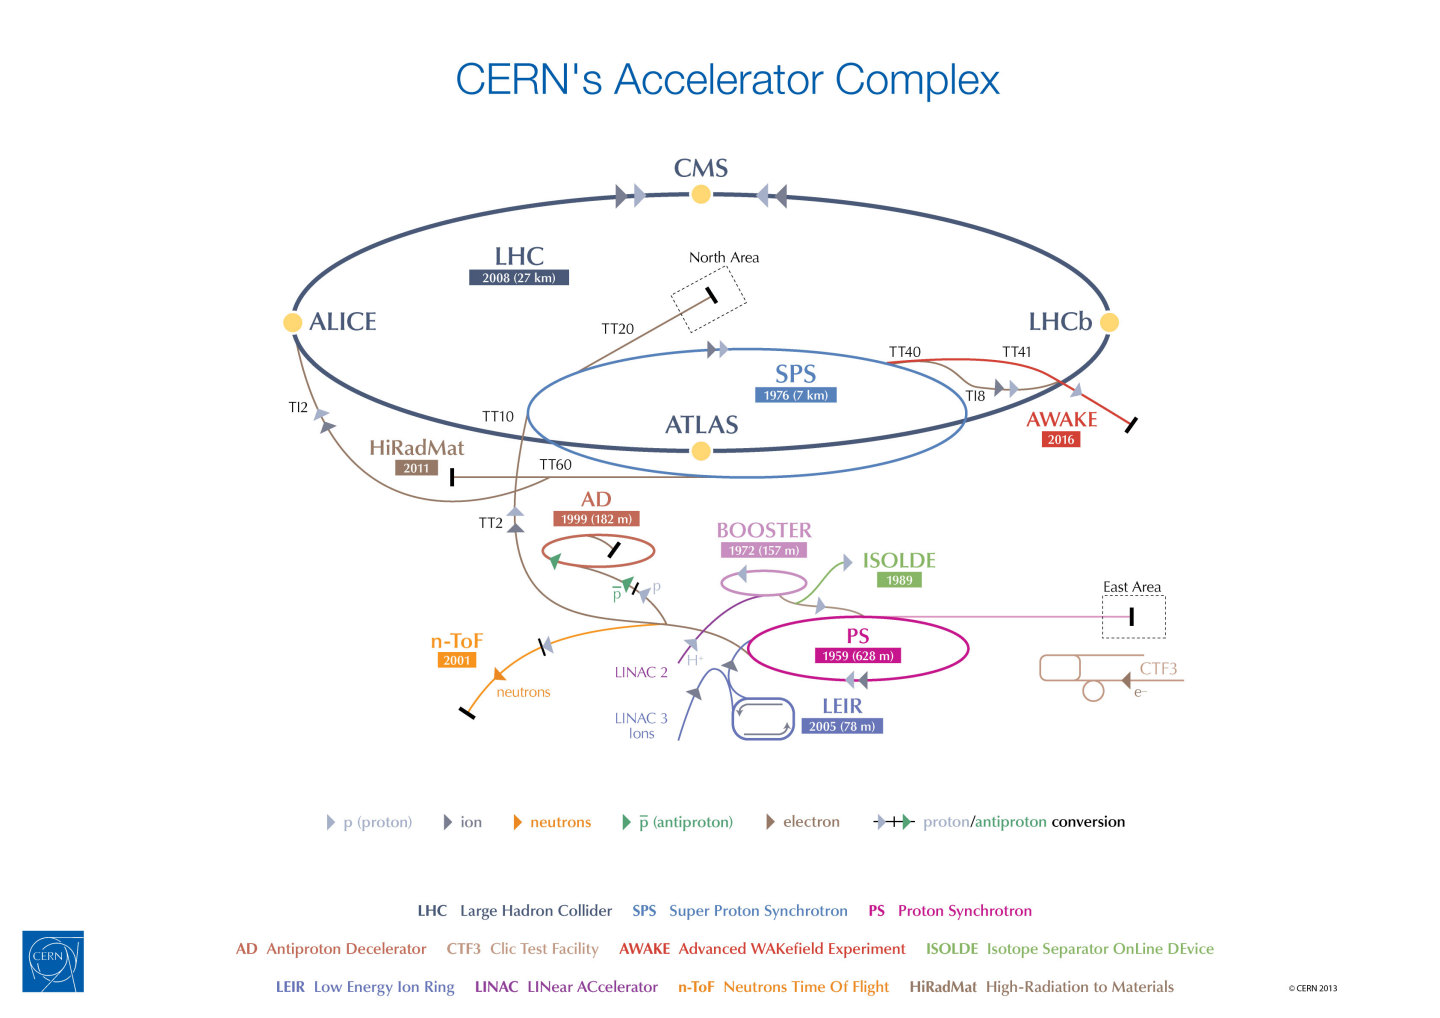
\includegraphics[scale=0.4]{CERN's-accelerator-complex2013.jpg}
\caption{The accelerator complex at CERN~\cite{Marcastel:1621583}.}
\label{fig:CERN_accelerator_complex}
\end{center}
\end{figure}

The protons are extracted by ionization from a hydrogen source and are accelerated to 50~{\MeV} by the linear accelerator LINAC2.
Then they are injected into the Proton Synchrotron Booster (PSB) where the proton energies are increased to 1.4~{\GeV} before they enter the Proton Synchrotron (PS) which accelerates the protons to 25~{\GeV}.
Next, the proton energies are increasing to 450~{\GeV} in the Super Proton Synchrotron (SPS). 
Finally, the protons are split into two beams and enter the LHC where the two beams run in two adjacent beam pipes with opposite directions.
In order to keep the protons on the circular trajectory in the LHC, 1232 superconducting dipole magnets~\cite{1288863} generate a magnetic field strength of 8.33~T to bend the proton beams in eight arcs.
Additionally, 392 quadrupole magnets~\cite{1288863} are installed to focus the beam.
A cryogenic system running with super-fluid helium-4 is used to cool down the superconducting magnets to a temperature of 1.7~K.

For a given physics process, the event rate is proportional to the cross section $\sigma$ of this process.
\begin{equation}
\frac{dN}{dt} = \mathcal{L}\cdot\sigma
\end{equation}
where $N$ is the number of events and $\mathcal{L}$ denotes the luminosity of the beam.
The luminosity of the beam, $\mathcal{L}$ can be calculated by
\begin{equation}
\mathcal{L} = \frac{N^{2} f}{4 \pi \sigma_{x} \sigma_{y}} \cdot F
\end{equation}
where $N$ is the number of protons, $f$ is the bunches crossing frequency, and the $\sigma_{x}$ and $\sigma_{y}$ are the $x$ and $y$ components for cross section $\sigma$.
The geometric luminosity reduction factor, $F$, is related to the crossing angle at the Interaction Point (IP).
Considering a beam consisting of $1.15 \times 10^{11}$ protons with bunching spacing of 25~ns, the transversal size of the bunch at Interaction Pointe $16\times 10^{-4}$~cm, and taking the geometric luminosity reduction factor as 1, the design luminosity of $10^{34}$~cm$^{-2}$s$^{-1}$ can be reached.

The first beam was circulated through the collider on the morning of 10 September 2008~\cite{CERN-COURIER-Sep192008}.
However, a magnet quench incident occurred on 19 September 2008 and caused extensive damage to over 50 superconducting magnets, their mountings, and the vacuum pipe.
Most of 2009 was spent on repairs the damage caused by the magnet quench incident and the operations resumed on 20 November of that year.
The first phase of data-taking (Run 1) started at the end of 2009 and the beam energy was increased to a centre-of-mass $\sqrt{s}=7$~{\TeV} in 2011 and $\sqrt{s} = 8$~{\TeV} in 2012.
The total integrated luminosity of 5.46~{\ifb} was collected in 2011 and of 22.8~{\ifb} was collected in 2012.
Since 13 February 2013 the LHC was in the Long Shutdown 1 (LS1) phase for maintenance and upgrades.
On 5 April 2015, the LHC restarted and was operating at a centre-of-mass energy $\sqrt{s}=13$~{\TeV} throughout the Run 2 phase\footnote{The Run 2 data-taking started from 2015}.


%%%%%
%%%%%
%%%%%

\section{The ATLAS experiment}

The ATLAS\footnote{A Toroidal LHC Apparatus} detector~\cite{1748-0221-3-08-S08003} is a multi-purpose detector housed in its cavern at point 1 at the LHC~\cite{1748-0221-3-08-S08001}.
It is the largest experiment at the LHC with a length of 44~m, a diameter of 25~m, and a weight of approximately 7000 tonnes.
It consists of three high precision sub-detector systems which are arranged concentrically around the interaction point and in forward and backward symmetrically.
Related to this symmetry, the ATLAS detector is sectioned into the central barrel region with one end-cap region perpendicular to the beam pipe on either side.
Figure~\ref{fig:ATLAS_detector} shows an overview of the ATLAS detector with its major components.

\begin{figure}[htbp]
\begin{center}
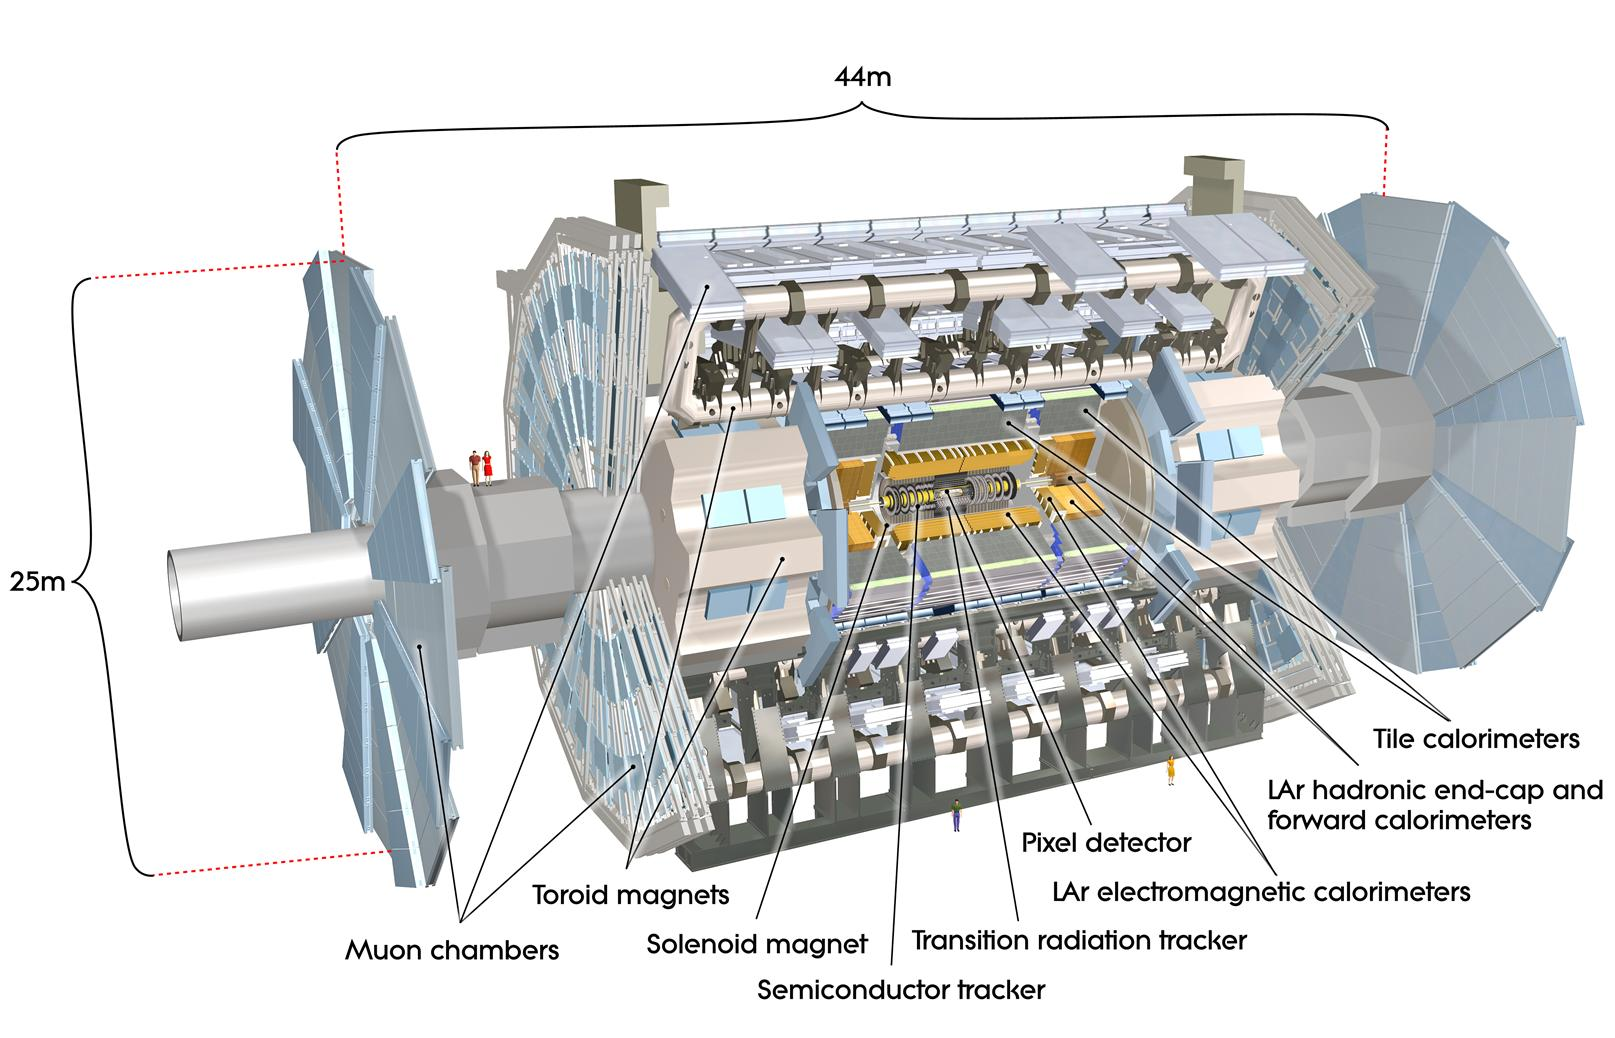
\includegraphics[scale=0.5]{0803012_01-A4-at-144-dpi.jpg}
\caption{Overview of the ATLAS detector~\cite{1748-0221-3-08-S08003}.}
\label{fig:ATLAS_detector}
\end{center}
\end{figure}

The ATLAS detector is designed to record the proton-proton interactions delivered by the LHC.
It can identify particles and measure their tracks and energies with very high precision, therefore, it is sensitive to large areas of particle physics phenomena from the precision measurement of the Standard Model (SM) to beyond the SM.
The detector is constituted by three sub-detector systems and the magnet system.
The innermost part of the detector is called the inner detector which identifies and reconstructs the charged particles as well as the primary and secondary vertices.
Around it, the calorimeter system is built as a cylindrical barrel with caps at each end to measure the particle energies.
The detector is completed by the muon spectrometer which performs identification and measurement of momenta of muons.
The magnetic system produces a field of $B$ = 0.5~T and $B$ = 1~T at barrel and two end-cap, respectively.
The detector has to withstand large collision rates with approximately 1000 particles per collision, therefore, a fast readout and a three-level trigger system are implemented to reduce the event rate from 40~MHz to 200~Hz.
The ATLAS coordinate system and the detail of each sub-detector systems are described in the following sections.

\subsection{The ATLAS coordinate system}

ATLAS uses a right-handed coordinate system with its origin at the nominal proton-proton interaction point (IP) in the centre of the detector and the $z$-axis along the beam pipe.
Along the $z$-axis the detector is divided into side-A (positive $z$) and side-C (negative $z$).
The positive $x$-axis is defined by the direction pointing from the IP to the centre of the LHC ring, and the positive $y$-axis points upward.%Cylindrical coordinates $(r, \phi)$ are used in the transverse plane.
The azimuthal angle $\phi$ is measured around the beam pipe  and the polar angle $\theta$ is the angle from the $z$-axis.
The transverse momentum $p_{\mathrm{T}}$, the transverse energy $E_{\mathrm{T}}$ and the missing transverse
energy $E_{\mathrm{T}}^{\mathrm{miss}}$ are defined in the transverse plane\footnote{$x-y$ plane}, here exemplary for $p_{\mathrm{T}}$:
%
\begin{equation}
p_{\mathrm{T}}= \sqrt{p_{x}^{2} + p_{y}^{2}}
\end{equation}
%
An important quantity in hadron collider physics is the \textbf{rapidity}, $y$, because of the invariance $y$ under Lorentz boosts in the longitudinal direction.
The rapidity is defined as
%
\begin{equation}
y = \frac{1}{2} \ln\Big[\frac{E + p_{z}}{E - p_{z}}\Big]
\end{equation}
%
where $E$ denotes the particle energy and $p_{z}$  is the component of the momentum along the beam direction.
Since mainly leptons can be considered massless in respect to the nominal centre-of-mass energy, the pseudorapidity, $\eta$, is used in stead of using the $y$.
For a massless particle, the \textbf{pseudorapidity}, $\eta$, depends on the polar angle $\theta$ through:
%
\begin{equation}
\eta = - \ln \tan \frac{\theta}{2}
\end{equation}
%
For a particle with the energy $E$ much larger than its mass, the approximation $E \approx |\vec{p}|$ is valid.
The distance, $\Delta R$, between two objects in the $\eta-\phi$ plan is given by
%
\begin{equation}
\Delta R = \sqrt{\Delta \eta^{2} + \Delta \phi^{2}}
\end{equation}
%
where $\Delta \eta$ and $\Delta \phi$ are the difference in pseudorapidity and azimuthal angle, respectively.

\subsection{The Inner Detector and Tracking System}
\label{subsec:inner_detector}

The Inner Detector (ID) consists of three sub-detectors: the Pixel detector, the silicon microstrip trackers  (SCT), and the Transition Radiation Tracker (TRT).
The main purpose of the ID is to provide high precision measurements of the tracks of particles and to reconstruct the primary and secondary vertices.
Each sub-detectors are composed of several layers of material which interacts with the charged particles when the charged particles penetrate the layers.
A  2~T magnetic field generated by the central solenoid parallel to the beam axis is applied to bend the charged particles using the Lorentz force.
By using the radius $r$ of the curvature of the tracks, the magnetic field strength $B$, and the charge of the particle $q$, we can calculate the magnitude of the transverse momentum \pt:
\begin{equation}
\pt = |q|Br
\end{equation}
The layout of the ID is illustrated in Figure~\ref{fig:Inner_detector} and the detail of sub-detectors are described in the following paragraphs.

\begin{figure}[htbp]
\begin{center}
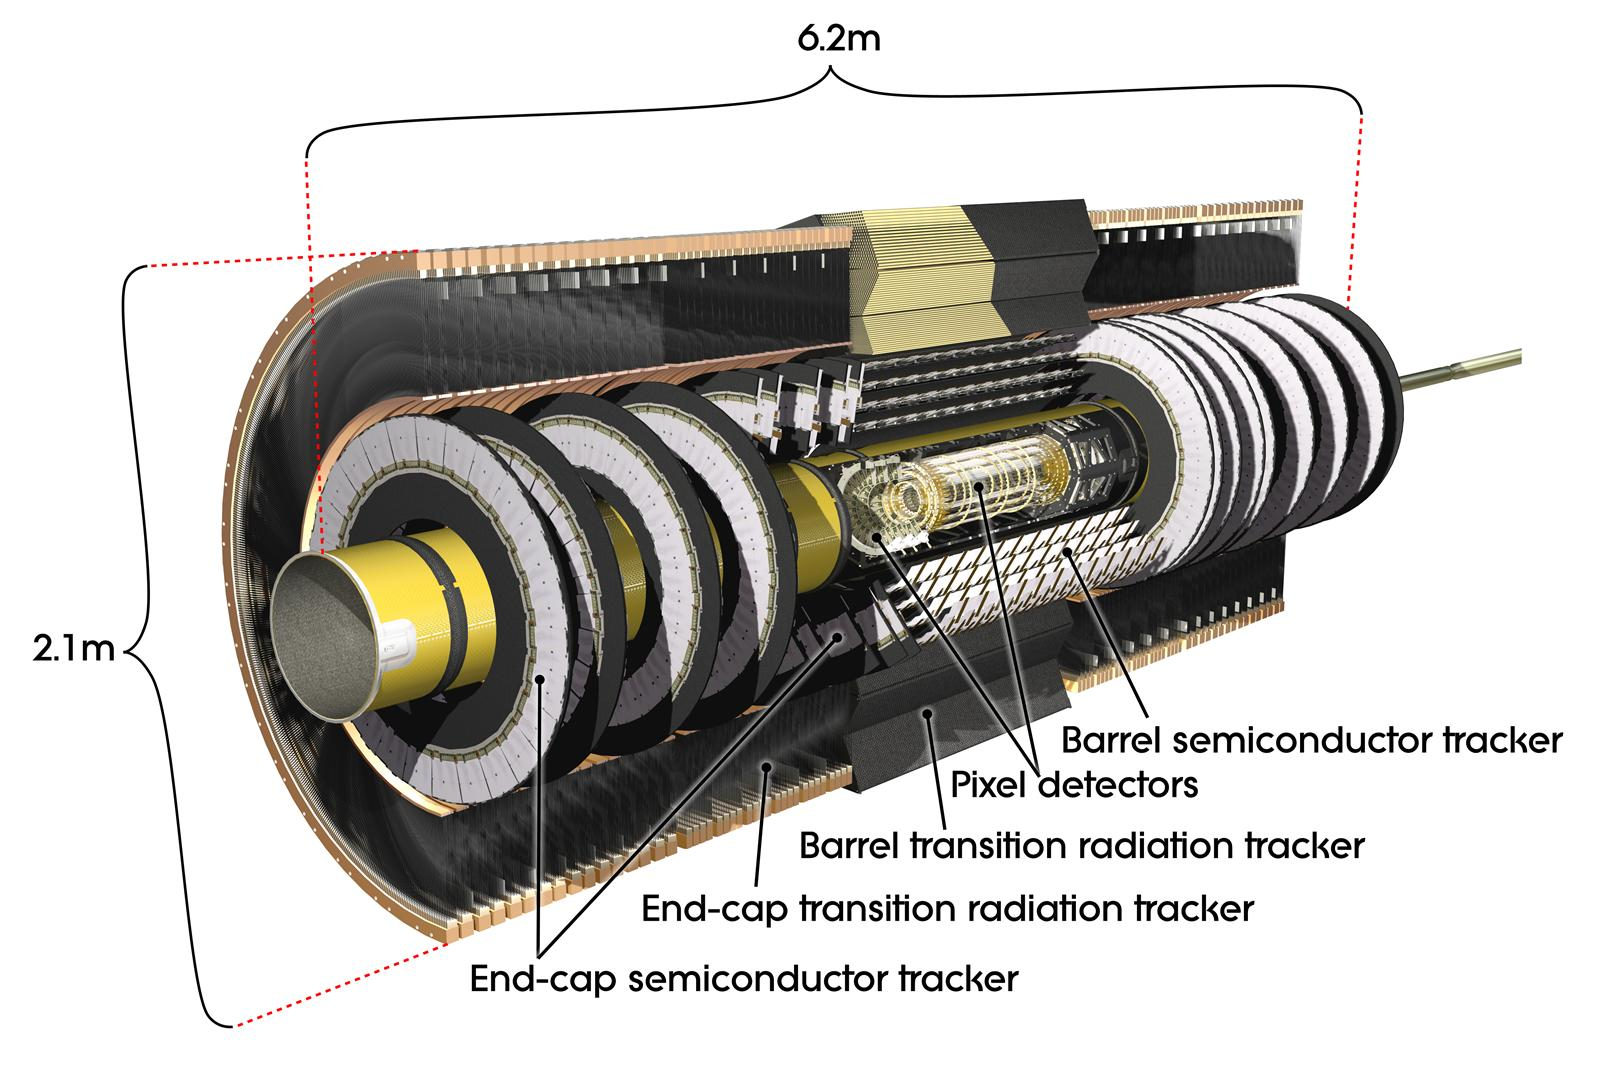
\includegraphics[scale=0.5]{0803014_01-A4-at-144-dpi.jpg}
\caption{Cut-away view of the ATLAS inner detector~\cite{1748-0221-3-08-S08003}.}
\label{fig:Inner_detector}
\end{center}
\end{figure}

%\subsubsection{Pixel Detector}
\noindent \textbf{Pixel Detector}

The innermost part of the entire ATLAS detector components is the Pixel detector which is composed of three barrel layers and three end-cap disks on each side.
The three cylindrical barrel layers around the beam axis have radial positions of 50.5~mm, 88.5~mm, and 122.5~mm respectively and they are made of 22, 38, and 52 identical staves respectively.
Each stave is inclined with azimuthal angle of 20 degrees and is composed of 13 pixel modules with 46,080 readout channel per module.
The size of each pixel is $50 \times 400~\mu m^{2}$ in $R-\phi \times z$.
In the forward region, three disks on each side equip the modules identical to the barrel modules, except the connecting cables. 
The total 1,744 modules in the pixel detector lead to nearly 80 million channel readout and provide the intrinsic accuracies of $10~\mu m$ in $R-\phi$ plane and $115~\mu m$ in $z$ direction covering the region $|\eta| < 2.5$. 

%\subsubsection{Semi Conductor Tracker}
\noindent \textbf{Semi Conductor Tracker}

On the top of the pixel detector is the Semi Conductor Tracker (SCT) which is a silicon strip detector.
There are about 6.3 million readout channels which are arranged in 4088 microstrips.
The intrinsic accuracies per sensor is $17~\mu m$ in $R-\phi$ and $580~\mu m$ in $z$ direction for the barrel and in $R$ for the  disks, respectively.
Similar to the pixel detector, the SCT covers the region $|\eta| < 2.5$ and consists of 8 strip layers in barrel and a total of 9 discs in the end-cap region on each side.
No track reconstruction is possible beyond the covered pseudorapidity range.
Therefore, the electrons cannot be distinguished from photons above $|\eta| > 2.5$ region.

%\subsubsection{Transition Radiation Tracker}
\noindent \textbf{Transition Radiation Tracker}

The outermost component of the ID is the Transition Radiation Tracker (TRT) which consists of 4~mm diameter straw tubes filled with the xenon-based gas mixture.
The gas mixture are ionized by charged particles when they penetrates the straws.
The ionized electrons drift to the cathode because a high voltage is applied on the tungsten wire in the center of the straw tube.
Therefore, the TRT allows the enhanced electron identification, momentum measurement, vertex measurement.
In the barrel region, the straws are surrounded by polypropylene fibres and are divided into two halves at $|\eta|=0$.
In the end-caps, the straws are arranged radially and surrounded by foils as a transition radiation element.
They are read out at two sides and at the center of the TRT with the total number of the readout channels of TRT are approximately 350,000.
The TRT only provides information in the $R-\phi$ plane with an intrinsic accuracy of 130~$\mu$m per straw and covers a range up to $|\eta| < 2.0$. 

%\subsubsection{Solenoid Magnet}
\noindent \textbf{Solenoid Magnet}

A superconducting solenoid magnet encloses the ID and produces a 2~T magnetic field to bend the trajectories of the charged particles.
A cooling system is used and shared with the electromagnetic calorimeter~\ref{subsec:calorimeter} to reduced the deterioration of the energy measurement.

\subsection{The Calorimeters}
\label{subsec:calorimeter}

The calorimeters are used to measure the energy of particles, such as electrons, photons, and jets.
Besides muons, all electromagnetically or haronically interacting particles are stopped in the calorimeters by absorbing their energy.
Not only charged particles but also neutral particles such as photons and neutral hadrons can be detected in the calorimeter.
By requiring highly hermiticity of the calorimeter, the missing energy can be reconstructed precisely as negative vectorial sum of all energy deposits.
The ATLAS Calorimeters system are placed between the Inner Detector~\ref{subsec:inner_detector} and the Muon Spectrometer~\ref{subsec:the_muon_spectrometer}.
The ATLAS calorimeters system consist of an inner Electromagnetic and outer Hadronic Calorimeter together with the Forward Calorimeter.
The Electromagnetic Calorimeter is dedicated for measuring electrons and photons, and the Hadronic Calorimeter focusing on hadronically interacting particles.
The calorimeters cover a range $|\eta| < 4.9$.
An layout view of the ATLAS Calorimeters system is shown in Figure~\ref{fig:calorimeter}

%\subsubsection{Electromagnetic Calorimeter}
\noindent \textbf{Electromagnetic Calorimeter}

The Electromagnetic Calorimeters (ECAL) measure the energy of electrons and photons as they interact with matter.
The ECAL consists of layers of high-density material, lead, as absorbers and interleaved with layers of liquid argon (LAr) as active medium.





%\subsubsection{Hadronic Calorimeter}
\noindent \textbf{Hadronic Calorimeter}


Hadrons, which are signi cantly heavier and mainly interact via the strong force, propagate further causing more wide-spread hadronic showers mainly in the denser Hadronic Calorimeter.

%\subsubsection{Forward Calorimeter}
\noindent \textbf{Forward Calorimeter}


\begin{figure}[htbp]
\begin{center}
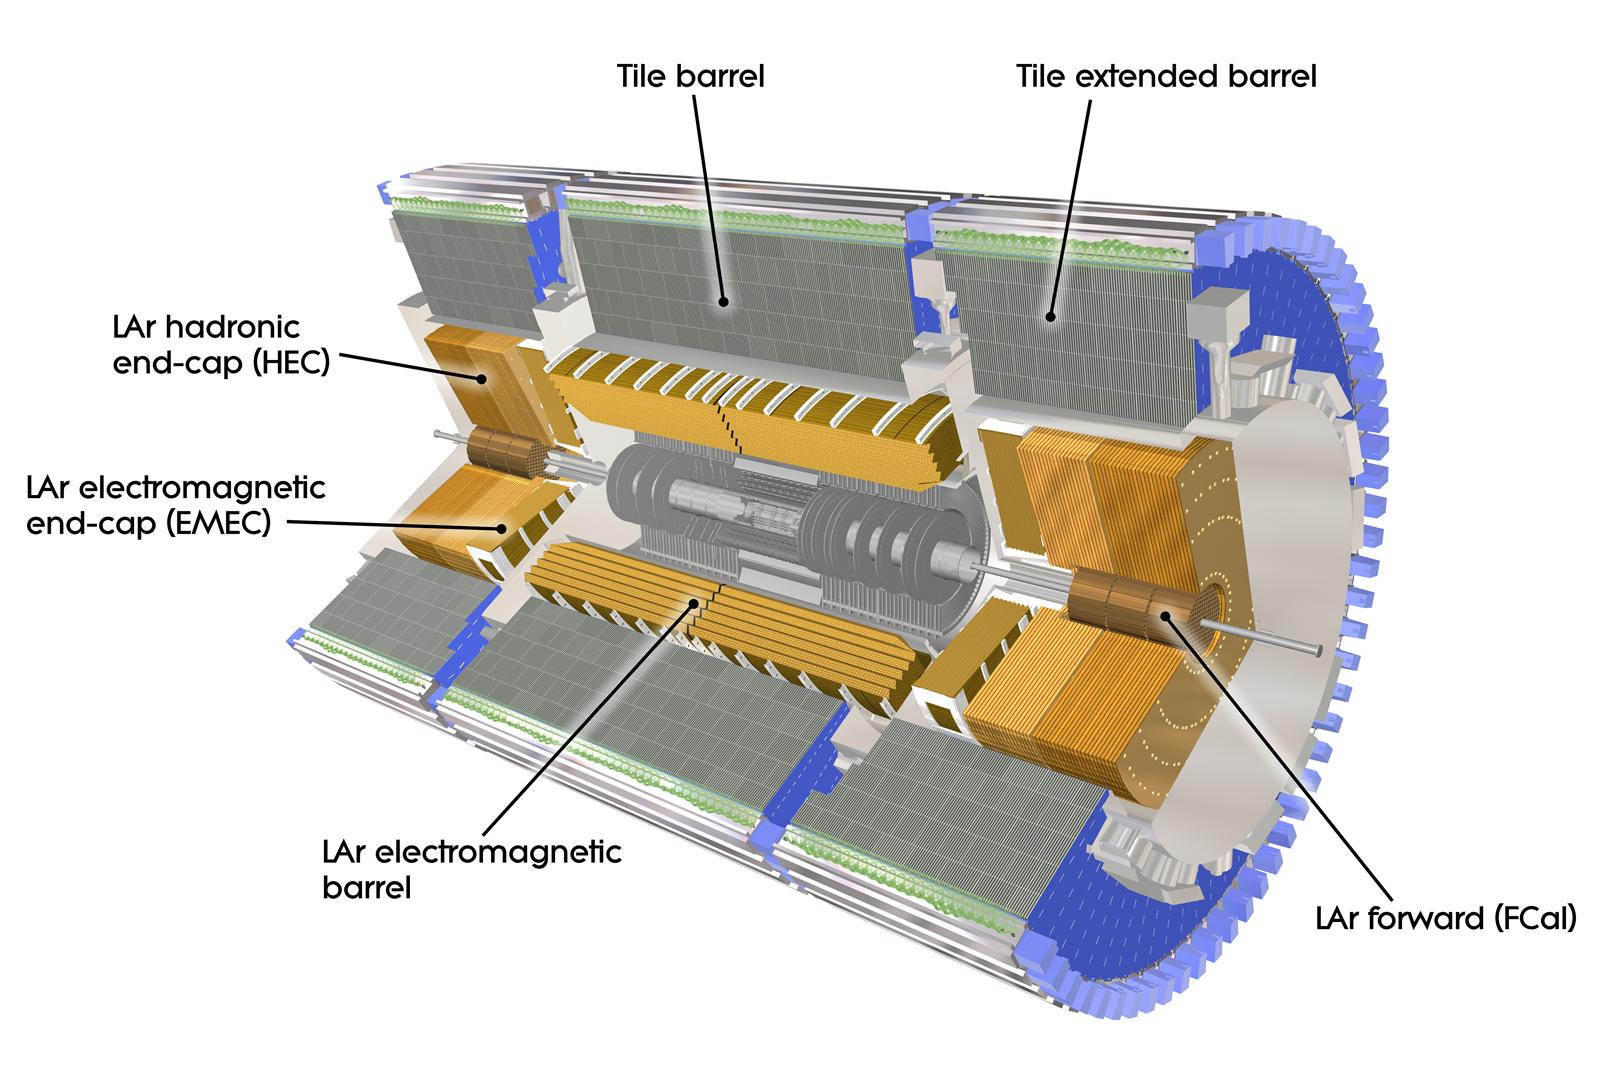
\includegraphics[scale=0.5]{0803015_01-A4-at-144-dpi.jpg}
\caption{Cut-away view of the calorimeter system~\cite{1748-0221-3-08-S08003}.}
\label{fig:calorimeter}
\end{center}
\end{figure}

\begin{table}[htbp]
\begin{center}
\begin{tabular}{cc}
\hline
\hline
Calorimeter & Required resolution\\
\hline
ElectromagneticCalorimeter & $\sigma_{E}/E = 10\% / \sqrt{E\mathrm{ (GeV)}} \oplus 0.7\%$\\
Hadronic Calorimeter & $\sigma_{E}/E = 50\% / \sqrt{E~\mathrm{(GeV)}} \oplus 3\%$\\
Forward Calorimeter & $\sigma_{E}/E = 100\% / \sqrt{E~\mathrm{(GeV)}} \oplus 10\%$\\
\hline
\hline
\end{tabular}
\end{center}
\caption{Resolution requirements for the different calorimeters of the ATLAS detector~\cite{1748-0221-3-08-S08003}.}
\label{tab:}
\end{table}%







\subsection{The Muon Spectrometer} \label{subsec:the_muon_spectrometer}

The outermost part of the ATLAS detector is the Muon Spectrometer~\cite{1748-0221-3-08-S08003}~\cite{Palestini:681459}~\cite{0910.2767}.
Muons have the same properties as electrons but 200 times heavier than the electrons and muons don't interact predominately by Bremsstrahlung but have minimal ionizing at LHC energy in the inner layers of the detector.
Only the muons with an energy less than 5~{\GeV} are stopped before the Muon Spectrometer.
Therefore, muons are the only measurable particles that can penetrate the Inner Detector and the Calorimeters.
In order to determine the muon momentum with high precision, a detector that concentrates on the measurement of muons is necessary.

The Muon Spectrometer is designed to measure the transverse momentum ($p_{\mathrm{T}}$) of muons with $p_{\mathrm{T}} > 3$~{\GeV} with a resolution of 3\% for $p_{\mathrm{T}} < 250$~{\GeV} and increasing to 10\% at 1~{\TeV}.
It consists of large toroid magnets system and three layers of high precision tracking chambers which allow a precise measurement of the muon momentum over nearly the full solid angle.
The barrel toroid magnet system is composed of eight superconducting coils which are installed radial symmetrically around the beam pipe.
It covers the range $|\eta| < 1.4$ and bends the trajectories of muons with the bending power 1.5 to 5.5 Tm.
The magnetic field produced by the barrel toroid magnets provides an approximately 1~T field at the center of each coils, but is rather non-uniform, especially in the barrel-endcap transition region.
In the endcap toroid magnets system, the magnetic field is provided by eight superconducting coils, closed in an insulation vessel extending to about 10 m in diameter, located between the first and the second station of tracking chambers.
The endcap toroid magnets cover $1.6 < |\eta| < 2.4$ and provide a a magnetic field in the range of 1 to 2 T with bending power 1 to 7.5 Tm.

The Monitored Drift Tubes (MDTs) consists of cylindrical drift tubes, filled with a gas mixture of argon and carbon dioxide.
A tungsten-rhenium alloyed aluminium wire in the centre of each tube collects the electrons freed by ionization of the gas volume by traversing muons.
The MDTs covers a full range of $|\eta| < 2.7$, while the inner layer only covers $|\eta| < 2.0$.
The Cathode Strip Chambers (CSCs) provides a coverage range $2.0 < |\eta| < 2.7$, where MDTs would have occupancy problems.
Both MDTs and CSCs are used for precision tracking in the spectrometer bending plane and end-cap inner layer, respectively.
The Resistive Plate Chambers (RPCs) and Thin Gap Chambers (TGCs) are used for triggering in barrel and end-cap, they have sufficient intrinsic time resolution of 1.5 ns and 4 ns, respectively.
A sketch of the Muon Spectrometer and its four components are depicted in Figure~\ref{fig:muon_spectrometer} and Table~\ref{tab:muon_spectrometer_components} gives a summary of the Muon Spectrometer components

\begin{figure}[htbp]
\begin{center}
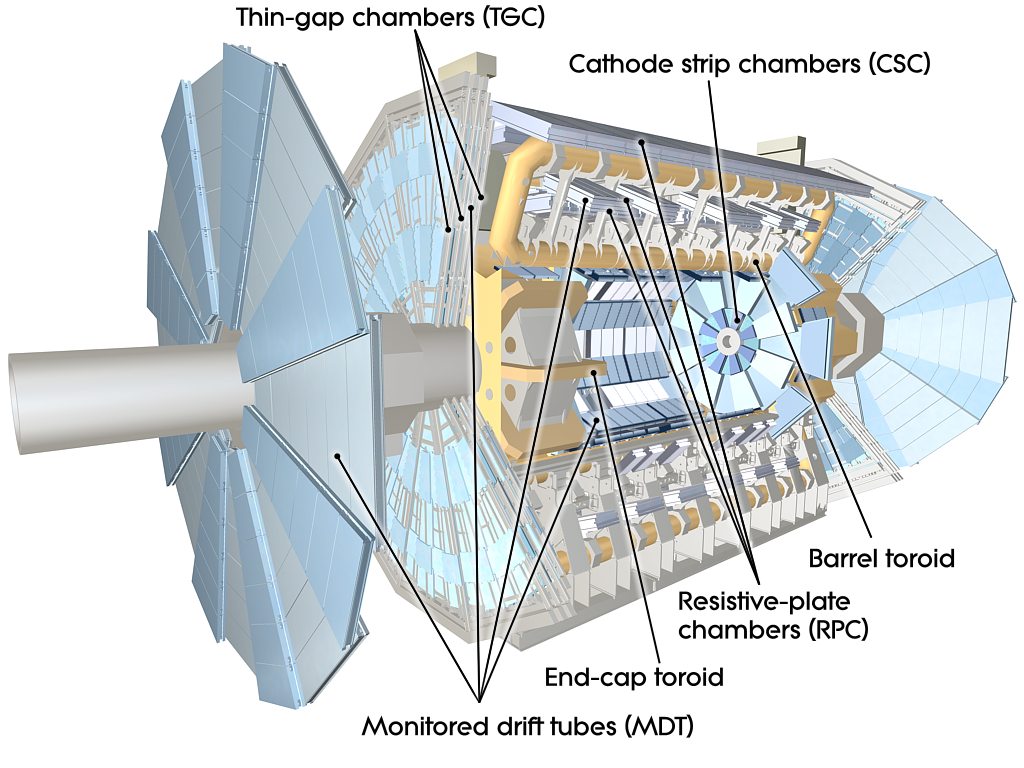
\includegraphics[scale=0.4]{MuonSystem_d3.png}
\caption{Sketch of the muon system of the ATLAS detector~\cite{1748-0221-3-08-S08003}.}
\label{fig:muon_spectrometer}
\end{center}
\end{figure}

\begin{table}[htbp]
\begin{center}
\begin{tabular}{ccccc}
\hline
\hline
Type & Purpose & Location & $\eta$ coverage & Channel\\
\hline
MDT & Tracking & barrel + end-cap & $0.0 < \eta < 2.7$ & 354k\\
CSC & Tracking & end-cap layer 1 & $2.0 < \eta < 2.7$ & 30.7k\\
RPC & Trigger & barrel & $0.0 < \eta < 1.0$ & 373k\\
TGC & Trigger & end-cap & $1.0 < \eta < 2.4$ & 318k\\
\hline
\hline
\end{tabular}
\end{center}
\caption{A summary of the Muon Spectrometer components.}
\label{tab:muon_spectrometer_components}
\end{table}%

\subsection{The Trigger System and Data Acquisition}

\subsection{}



%\chapter{The Electron Isolation Efficiency and Scale Factors}
%\label{chapter:electron_isolation}
%\graphicspath{{figures/electron_isolation}}
%\input{chapter_electron_isolation}


%\chapter{The Real Lepton Efficiencies}
%\label{chapter:real_lepton_efficiencies}
%\graphicspath{{figures/real_lepton_efficiencies}}
%\input{chapter_real_lepton_efficiencies}

%\chapter{Results}
%\label{chapter:results}
%\graphicspath{{figures/results/}}
%A search for the electroweak production of supersymmetric states with low \pt visible decay products is presented.
Events with significant \met and same flavor opposite charged lepton pairs are selected.
The minimum \pt of the lepton is 4.5~{\GeV} for the electrons and 4~{\GeV} for the muons.
The dilepton invariant mass and stranverse mass are the main discriminating variables used to construct signal regions.
This analysis is performed using LHC proton-proton collision data at $\sqrt{s} = 13$~{\TeV} collected by the ATLAS detector corresponding to an integrated luminosity of 36.1~\ifb.
Since no excess over the Standard Model expectation is observed, the results are interpreted using $R$-parity-conserving supersymmetry, where the produced states have small mass splitting with the lightest neutralino $\widetilde{\chi}^{0}_{1}$.
For the NUHM2 scenario, 95\% CL cross-section upper limits ranging between 11.5 and 3.8 pb for $m_{1/2}$ values of 350 to 800~{\GeV} are provided.


%\FloatBarrier

%\chapter{Conclusion}
%\label{chapter:conclusion}
%\graphicspath{{figures/conclusion/}}
%A search for the electroweak production of supersymmetric states with low \pt visible decay products is presented.
Events with significant \met and same flavor opposite charged lepton pairs are selected.
The minimum \pt of the lepton is 4.5~{\GeV} for the electrons and 4~{\GeV} for the muons.
The dilepton invariant mass and stranverse mass are the main discriminating variables used to construct signal regions.
This analysis is performed using LHC proton-proton collision data at $\sqrt{s} = 13$~{\TeV} collected by the ATLAS detector corresponding to an integrated luminosity of 36.1~\ifb.
Since no excess over the Standard Model expectation is observed, the results are interpreted using $R$-parity-conserving supersymmetry, where the produced states have small mass splitting with the lightest neutralino $\widetilde{\chi}^{0}_{1}$.
For the NUHM2 scenario, 95\% CL cross-section upper limits ranging between 11.5 and 3.8 pb for $m_{1/2}$ values of 350 to 800~{\GeV} are provided.


%------------------------------------------------------------------------------- 
\clearpage

%\appendix
%\part*{Appendix}
%\addcontentsline{toc}{part}{Appendix}

%\section{Simulated samples, cross-sections and equivalent luminosities}
%\label{app:samples}
%The Monte Carlo (MC) samples are used to model the SUSY signals and to estimate the SM background.
The MC samples are processed using a ATLAS detector full simulation (FullSim) or a fast simulation (AFII\footnote{AFII stands for ATLAS Fast II.}) based on {\GEANT}4~\cite{Agostinelli:2002hh} simulation package.
The FullSim simulates the detailed properties of the ATLAS detector while the AFII uses a parameterized calorimeter response and simulates ID and MS~\cite{ATLAS:1300517} based on {\GEANT}4.
The simulated MC events are reweighted to the observed pile-up conditions in the data.

%%%
%%%
%%%

\section{Samples used for strong interaction}
\label{sec:app_samples_strong}

Table~\ref{tab:app_sample_strong} shows the event generator, parton shower, cross-section normalization, PDF set~\cite{Martin:2009iq}, and the set of tunned parameters for modelling for all samples.
Except those produced by the {\SHERPA}, the \textsc{EvtGEN}\xspace v1.2.0 package~\cite{Lange:2001uf} is used to model the properties of bottom and charm hadron decays for all MC samples.

\begin{table}[htp]
%\begin{center}
\resizebox{\textwidth}{!}{% <------ Don't forget this %
\begin{tabular}{ccccccc}
\hline
\hline
Signal/Background                                      & Physics process                   & Event generator                  & Parton shower     & Cross-section normalization & PDF set    & Set of tunned parameters\\
\hline
\hline
\multirow{3}{*}{Signal}                                & RPC                               & MG5\_{\scriptsize A}MC@NLO 2.2.3 & {\PYTHIA} 8.186   & NLO+NLL                     & NNPDF2.3LO & A14\\
                                                       & RPV (except Figure~\ref{})        & MG5\_{\scriptsize A}MC@NLO 2.2.3 & {\PYTHIA} 8.210   & or                          & NNPDF2.3LO & A14\\
                                                       & RPV (Figure~\ref{})               & {\HERWIGpp} 2.7.1                & {\HERWIGpp} 2.7.1 & NLO-Prospino2               & CTEQ6L1    & UEEE5\\
\hline
\multirow{3}{*}{\shortstack{$t\bar{t}+X$\\background}} & $t\bar{t}W, t\bar{t}Z/\gamma^{*}$ & MG5\_{\scriptsize A}MC@NLO 2.2.2 & {\PYTHIA} 8.186   & NLO                         & NNPDF2.3LO & A14\\
                                                       & $t\bar{t}H$                       & MG5\_{\scriptsize A}MC@NLO 2.3.2 & {\PYTHIA} 8.186   & NLO                         & NNPDF2.3LO & A14\\
                                                       & 4$t$                              & MG5\_{\scriptsize A}MC@NLO 2.2.2 & {\PYTHIA} 8.186   & NLO                         & NNPDF2.3LO & A14\\
\hline
\multirow{2}{*}{\shortstack{Dibosno\\background}}      & $ZZ, WZ$                          & {\SHERPA} 2.2.1                  & {\SHERPA} 2.2.1   & NLO                         & NNPDF2.3LO & {\SHERPA} default\\
                                                       & Other (inc. $W^{\pm}W^{\pm}$)     & {\SHERPA} 2.1.1                  & {\SHERPA} 2.1.1   & NLO                         & CT10       & {\SHERPA} default\\
\hline
\multirow{4}{*}{\shortstack{Rare\\background}}         & $t\bar{t}WW, t\bar{t}WZ$          & MG5\_{\scriptsize A}MC@NLO 2.2.2 & {\PYTHIA} 8.186   & NLO                         & NNPDF2.3LO & A14\\
                                                       & $tZ, tWZ, tt\bar{t}$              & MG5\_{\scriptsize A}MC@NLO 2.2.2 & {\PYTHIA} 8.186   & LO                          & NNPDF2.3LO & A14\\
                                                       & $WH, ZH$                          & MG5\_{\scriptsize A}MC@NLO 2.2.2 & {\PYTHIA} 8.186   & NLO                         & NNPDF2.3LO & A14\\
                                                       & Triboson                          & {\SHERPA} 2.1.1                  & {\SHERPA} 2.1.1   & NLO                         & CT10       & {\SHERPA} default\\
\hline
\hline
\end{tabular}
%\end{center}
}
\caption{The simulated signal and background MC samples.
The event generator, parton shower, cross-section normalization, PDF set, and the set of tunned parameters for each samples are shown.
The $t\bar{t}WW, t\bar{t}WZ, tZ, tWZ, tt\bar{t}, WH, ZH$ and triboson background samples are labeled in the "rare" because they contribute a very small amount to the signal region.}
\label{tab:app_sample_strong}
\end{table}%


%%%
%%%
%%%

\section{Samples used for weak interaction}
\label{sec:app_samples}

%%%
%%%
%%%
%\clearpage
%-------------------------------------------------------------------------------

\clearpage

%\printbibliography
\clearpage










\bibliographystyle{unsrt}
%% You need a file named `outhesis_references.bib' to use BibTex here
%\bibliography{outhesis_references}
\bibliography{bib_standard_model,bib_atlas_experiment}
%\bibliography{}



% \appendix{A}
% \input{appendices/appendixA}
%\begin{appendices}
%\input{chapter_hardware}
%\input{chapter_auxiliaryPlots8TeV}
%\input{chapter_JSSuncSmoothing}
%\end{appendices}


% \backmatter


\end{document}

